\documentclass[../master]{subfiles}
\begin{document}

\chapter{iso-C$_{\text 4}$H$_{\text{10}}$ (10) + H$_{\text 2}$ (9)を用いたとき}
本章では検出ガスとして用いる\isoButaneHydro の特性について述べる.
\section{ドリフトスピード}
ドリフトスピードのドリフト電場依存性を調べた.
Magboltz でドリフトスピードが\SI{0.014}{\milli\metre\per\nano\second}となる
ドリフト電場は\SI{6.80}{\volt\per\milli\metre}である.
ドリフト領域の長さは\SI{140}{\milli\metre}であるので,plateとgridの電位差は\SI{952}{\volt}となる.
調整の行いやすさを考え\SI{955}{\volt}を中心に\SI{100}{\volt}間隔で
\SIrange{455}{1455}{\volt}の範囲で変化させて計10点測定した.
線源を用いて測定したドリフトスピードとMagboltz により求めたドリフトスピードを図\ref{fig::drift_speed_E_dep}に示す.
\begin{figure}
  \centering
  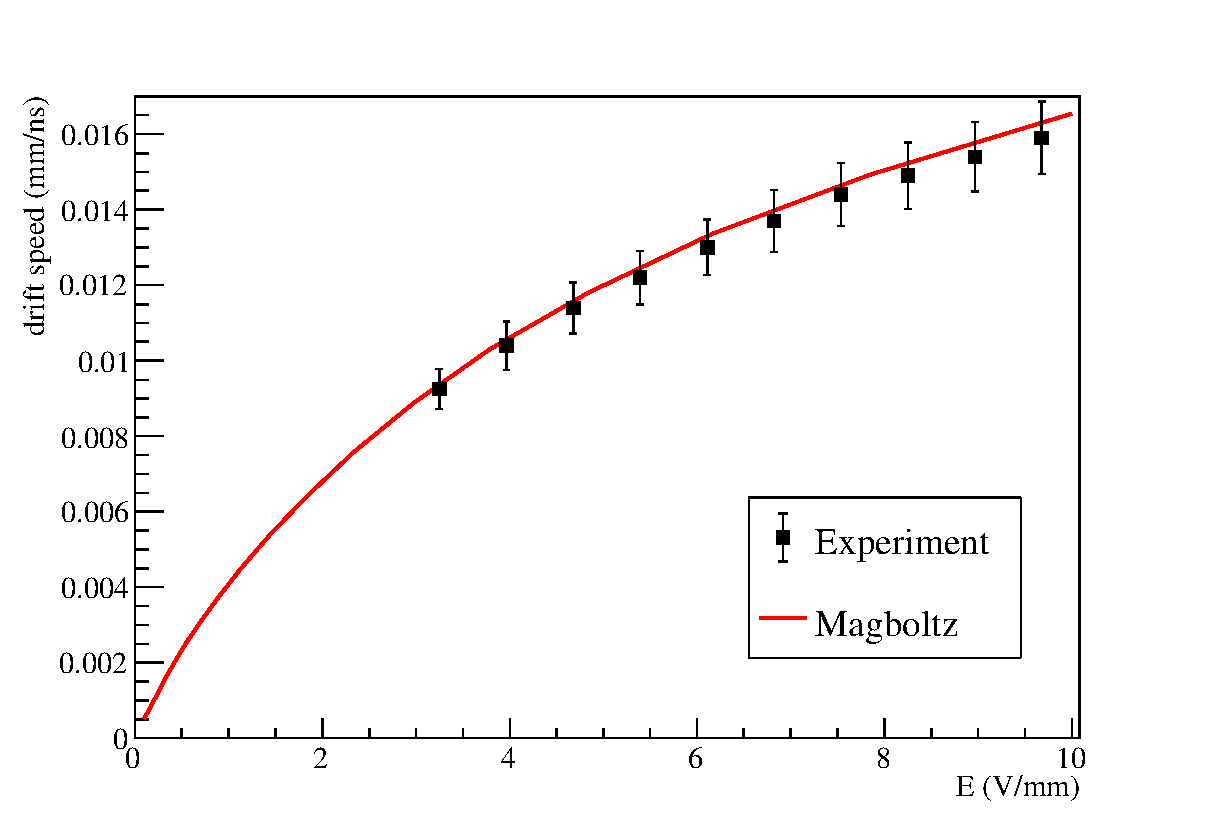
\includegraphics[clip, width=0.8\columnwidth]{drift_E_dep.eps}
  \caption{ドリフトスピードの電場依存性.点は測定したドリフトスピード,実線はMagboltz で求めたドリフトスピードを示す.}
  \label{fig::drift_speed_E_dep}
\end{figure}
線源を用いて測定したドリフトスピードと Magboltz で求めたドリフトスピードがおよそ一致していることが分かる.
ただ,全体的に測定値のドリフトスピードの方が小さくなている.
これは測定で用いた検出ガスに水分などの不純物が含まれていることが原因と考えられる.
水分によるドリフトスピードの変化は付録\ref{app::drift_speed_humid_dep}で述べる.

\section{電子増幅率}
電子の増幅率はGEM,$\mu$-PICの電圧によって変化する.
また,gridやGEMを通過する際に電子の一部が増幅されずに吸収されてしまう.
そこで,電子増幅率の電位差依存性を調べる.
grid とGEM との電位差を$\Delta V_{\text{grid-GEM}}$, GEMの両面間の電位差を$\Delta V_{\text{GEM}}$,
GEM の$\mu$-PIC側と$\mu$-PICとの電位差を$\Delta V_{\text{GEM-}\mu\text{-PIC}}$,
$\mu$-PICのanode 電極の電圧を$V_{\mu\text{-PIC}}$とする.
$\mu$-PICのcathode 電極は接地されている.
\begin{table}
  \centering
  \caption{基準となる電圧構成.}
  \label{tab::voltage_configuration}
%  \begin{tabular}{cc}
%    \toprule
%    & 電圧 (\si{\volt})\\
%    \midrule
%    plate & -2255 \\
%    grid & -1300 \\
%    GEM (top) & -600 \\
%    GEM (bottom) & -250 \\
%    $\mu$-PIC & 400\\
%    \bottomrule 
%  \end{tabular}
%\end{table}
%\begin{table}
%  \centering
%  \caption{}
%  
  \begin{tabular}{cc}
    \toprule
    項目 & 電位差 (\si{\volt}) \\
    \midrule
    $\Delta V_{\text{grid-GEM}}$ & 700 \\
    $\Delta V_{\text{GEM}}$ & 350 \\
    $\Delta V_{\text{GEM-}\mu\text{-PIC}}$ & 650 \\
    $V_{\mu\text{-PIC}}$ & 400 \\
    \bottomrule
  \end{tabular}
\end{table}
表\ref{tab::voltage_configuration}にあるような電位差を基準として,
各項目の電位差依存性を調べた.
表\ref{tab::voltage_configuration}は\ref{chap::simulation}章でドリフトスピードを測定したときの構成である.
増幅率の測定方法は\ref{chap::simulation}章で述べた通りである.
本測定ではGEM,$\mu$-PICの増幅率や電子の収集効率をそれぞれで求めることができないので,
それらを畳み込んだ増幅率として求める.

%ここで,GEMのうちgrid側をtop, $\mu$-PIC側をbottomと呼ぶ.

\subsection{gridとGEMとの電位差による電子の増幅率}
gridとGEMの間の電位差によって電子がドリフト領域から増幅領域へ移動する効率が変化することがわかっている~\cite{furuno}.
$\Delta V_{\text{grid-GEM}}$を\SI{20}{\volt}間隔で\SI{600}{}--\SI{780}{\volt}の範囲で変化させて計10点測定した.
電子の増幅率の$\Delta V_{\text{grid-GEM}}$による変化を図\ref{fig::gain_grid_GEM_V_dep}に示す.
\begin{figure}
  \centering
%  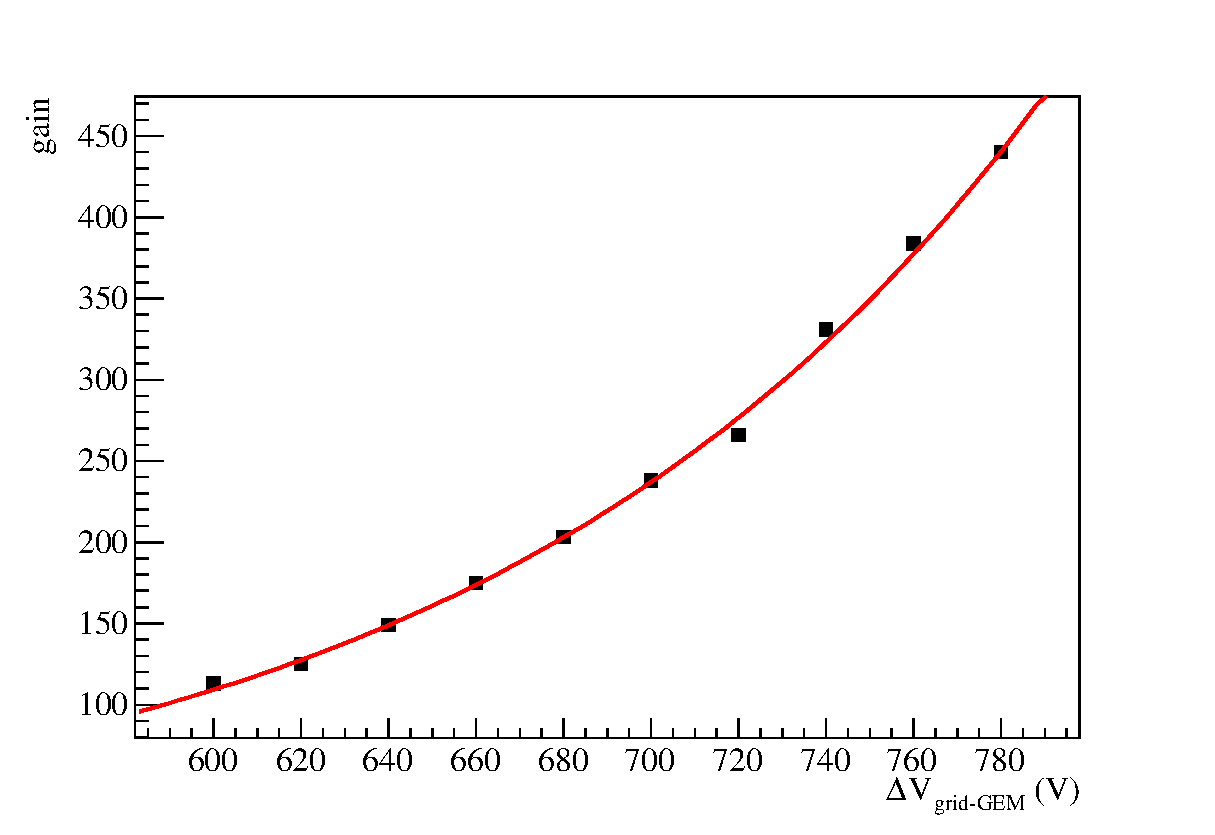
\includegraphics[clip, width=0.8\columnwidth]{gain_grid_V_dep_fit.eps}
  \scalebox{0.7}{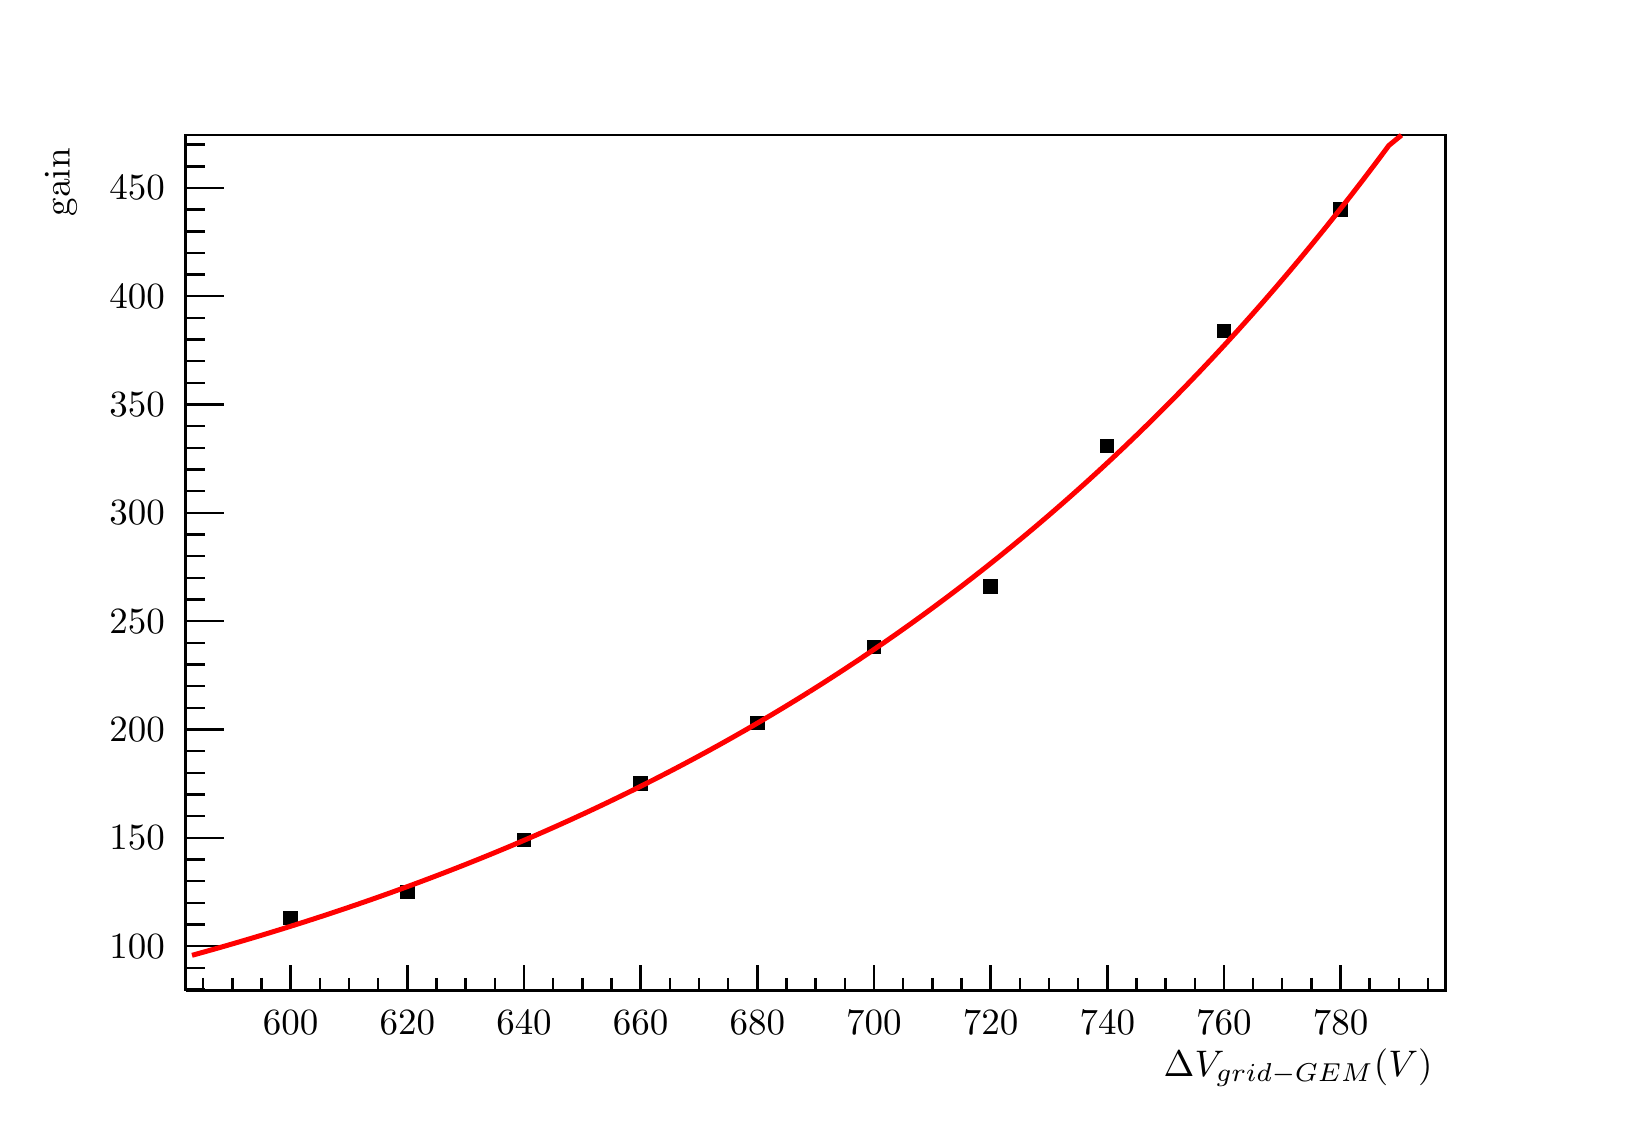
\begin{tikzpicture}
\pgfdeclareplotmark{cross} {
\pgfpathmoveto{\pgfpoint{-0.3\pgfplotmarksize}{\pgfplotmarksize}}
\pgfpathlineto{\pgfpoint{+0.3\pgfplotmarksize}{\pgfplotmarksize}}
\pgfpathlineto{\pgfpoint{+0.3\pgfplotmarksize}{0.3\pgfplotmarksize}}
\pgfpathlineto{\pgfpoint{+1\pgfplotmarksize}{0.3\pgfplotmarksize}}
\pgfpathlineto{\pgfpoint{+1\pgfplotmarksize}{-0.3\pgfplotmarksize}}
\pgfpathlineto{\pgfpoint{+0.3\pgfplotmarksize}{-0.3\pgfplotmarksize}}
\pgfpathlineto{\pgfpoint{+0.3\pgfplotmarksize}{-1.\pgfplotmarksize}}
\pgfpathlineto{\pgfpoint{-0.3\pgfplotmarksize}{-1.\pgfplotmarksize}}
\pgfpathlineto{\pgfpoint{-0.3\pgfplotmarksize}{-0.3\pgfplotmarksize}}
\pgfpathlineto{\pgfpoint{-1.\pgfplotmarksize}{-0.3\pgfplotmarksize}}
\pgfpathlineto{\pgfpoint{-1.\pgfplotmarksize}{0.3\pgfplotmarksize}}
\pgfpathlineto{\pgfpoint{-0.3\pgfplotmarksize}{0.3\pgfplotmarksize}}
\pgfpathclose
\pgfusepathqstroke
}
\pgfdeclareplotmark{cross*} {
\pgfpathmoveto{\pgfpoint{-0.3\pgfplotmarksize}{\pgfplotmarksize}}
\pgfpathlineto{\pgfpoint{+0.3\pgfplotmarksize}{\pgfplotmarksize}}
\pgfpathlineto{\pgfpoint{+0.3\pgfplotmarksize}{0.3\pgfplotmarksize}}
\pgfpathlineto{\pgfpoint{+1\pgfplotmarksize}{0.3\pgfplotmarksize}}
\pgfpathlineto{\pgfpoint{+1\pgfplotmarksize}{-0.3\pgfplotmarksize}}
\pgfpathlineto{\pgfpoint{+0.3\pgfplotmarksize}{-0.3\pgfplotmarksize}}
\pgfpathlineto{\pgfpoint{+0.3\pgfplotmarksize}{-1.\pgfplotmarksize}}
\pgfpathlineto{\pgfpoint{-0.3\pgfplotmarksize}{-1.\pgfplotmarksize}}
\pgfpathlineto{\pgfpoint{-0.3\pgfplotmarksize}{-0.3\pgfplotmarksize}}
\pgfpathlineto{\pgfpoint{-1.\pgfplotmarksize}{-0.3\pgfplotmarksize}}
\pgfpathlineto{\pgfpoint{-1.\pgfplotmarksize}{0.3\pgfplotmarksize}}
\pgfpathlineto{\pgfpoint{-0.3\pgfplotmarksize}{0.3\pgfplotmarksize}}
\pgfpathclose
\pgfusepathqfillstroke
}
\pgfdeclareplotmark{newstar} {
\pgfpathmoveto{\pgfqpoint{0pt}{\pgfplotmarksize}}
\pgfpathlineto{\pgfqpointpolar{44}{0.5\pgfplotmarksize}}
\pgfpathlineto{\pgfqpointpolar{18}{\pgfplotmarksize}}
\pgfpathlineto{\pgfqpointpolar{-20}{0.5\pgfplotmarksize}}
\pgfpathlineto{\pgfqpointpolar{-54}{\pgfplotmarksize}}
\pgfpathlineto{\pgfqpointpolar{-90}{0.5\pgfplotmarksize}}
\pgfpathlineto{\pgfqpointpolar{234}{\pgfplotmarksize}}
\pgfpathlineto{\pgfqpointpolar{198}{0.5\pgfplotmarksize}}
\pgfpathlineto{\pgfqpointpolar{162}{\pgfplotmarksize}}
\pgfpathlineto{\pgfqpointpolar{134}{0.5\pgfplotmarksize}}
\pgfpathclose
\pgfusepathqstroke
}
\pgfdeclareplotmark{newstar*} {
\pgfpathmoveto{\pgfqpoint{0pt}{\pgfplotmarksize}}
\pgfpathlineto{\pgfqpointpolar{44}{0.5\pgfplotmarksize}}
\pgfpathlineto{\pgfqpointpolar{18}{\pgfplotmarksize}}
\pgfpathlineto{\pgfqpointpolar{-20}{0.5\pgfplotmarksize}}
\pgfpathlineto{\pgfqpointpolar{-54}{\pgfplotmarksize}}
\pgfpathlineto{\pgfqpointpolar{-90}{0.5\pgfplotmarksize}}
\pgfpathlineto{\pgfqpointpolar{234}{\pgfplotmarksize}}
\pgfpathlineto{\pgfqpointpolar{198}{0.5\pgfplotmarksize}}
\pgfpathlineto{\pgfqpointpolar{162}{\pgfplotmarksize}}
\pgfpathlineto{\pgfqpointpolar{134}{0.5\pgfplotmarksize}}
\pgfpathclose
\pgfusepathqfillstroke
}
\definecolor{c}{rgb}{1,1,1};
\draw [color=c, fill=c] (0,0) rectangle (20,13.5817);
\draw [color=c, fill=c] (2,1.35817) rectangle (18,12.2235);
\definecolor{c}{rgb}{0,0,0};
\draw [c,line width=0.9] (2,1.35817) -- (2,12.2235) -- (18,12.2235) -- (18,1.35817) -- (2,1.35817);
\draw [c,line width=0.9] (2,1.35817) -- (18,1.35817);
\draw [c,line width=0.9] (3.33333,1.68413) -- (3.33333,1.35817);
\draw [c,line width=0.9] (3.7037,1.52115) -- (3.7037,1.35817);
\draw [c,line width=0.9] (4.07407,1.52115) -- (4.07407,1.35817);
\draw [c,line width=0.9] (4.44444,1.52115) -- (4.44444,1.35817);
\draw [c,line width=0.9] (4.81482,1.68413) -- (4.81482,1.35817);
\draw [c,line width=0.9] (5.18519,1.52115) -- (5.18519,1.35817);
\draw [c,line width=0.9] (5.55556,1.52115) -- (5.55556,1.35817);
\draw [c,line width=0.9] (5.92593,1.52115) -- (5.92593,1.35817);
\draw [c,line width=0.9] (6.2963,1.68413) -- (6.2963,1.35817);
\draw [c,line width=0.9] (6.66667,1.52115) -- (6.66667,1.35817);
\draw [c,line width=0.9] (7.03704,1.52115) -- (7.03704,1.35817);
\draw [c,line width=0.9] (7.40741,1.52115) -- (7.40741,1.35817);
\draw [c,line width=0.9] (7.77778,1.68413) -- (7.77778,1.35817);
\draw [c,line width=0.9] (8.14815,1.52115) -- (8.14815,1.35817);
\draw [c,line width=0.9] (8.51852,1.52115) -- (8.51852,1.35817);
\draw [c,line width=0.9] (8.88889,1.52115) -- (8.88889,1.35817);
\draw [c,line width=0.9] (9.25926,1.68413) -- (9.25926,1.35817);
\draw [c,line width=0.9] (9.62963,1.52115) -- (9.62963,1.35817);
\draw [c,line width=0.9] (10,1.52115) -- (10,1.35817);
\draw [c,line width=0.9] (10.3704,1.52115) -- (10.3704,1.35817);
\draw [c,line width=0.9] (10.7407,1.68413) -- (10.7407,1.35817);
\draw [c,line width=0.9] (11.1111,1.52115) -- (11.1111,1.35817);
\draw [c,line width=0.9] (11.4815,1.52115) -- (11.4815,1.35817);
\draw [c,line width=0.9] (11.8519,1.52115) -- (11.8519,1.35817);
\draw [c,line width=0.9] (12.2222,1.68413) -- (12.2222,1.35817);
\draw [c,line width=0.9] (12.5926,1.52115) -- (12.5926,1.35817);
\draw [c,line width=0.9] (12.963,1.52115) -- (12.963,1.35817);
\draw [c,line width=0.9] (13.3333,1.52115) -- (13.3333,1.35817);
\draw [c,line width=0.9] (13.7037,1.68413) -- (13.7037,1.35817);
\draw [c,line width=0.9] (14.0741,1.52115) -- (14.0741,1.35817);
\draw [c,line width=0.9] (14.4444,1.52115) -- (14.4444,1.35817);
\draw [c,line width=0.9] (14.8148,1.52115) -- (14.8148,1.35817);
\draw [c,line width=0.9] (15.1852,1.68413) -- (15.1852,1.35817);
\draw [c,line width=0.9] (15.5556,1.52115) -- (15.5556,1.35817);
\draw [c,line width=0.9] (15.9259,1.52115) -- (15.9259,1.35817);
\draw [c,line width=0.9] (16.2963,1.52115) -- (16.2963,1.35817);
\draw [c,line width=0.9] (16.6667,1.68413) -- (16.6667,1.35817);
\draw [c,line width=0.9] (3.33333,1.68413) -- (3.33333,1.35817);
\draw [c,line width=0.9] (2.96296,1.52115) -- (2.96296,1.35817);
\draw [c,line width=0.9] (2.59259,1.52115) -- (2.59259,1.35817);
\draw [c,line width=0.9] (2.22222,1.52115) -- (2.22222,1.35817);
\draw [c,line width=0.9] (16.6667,1.68413) -- (16.6667,1.35817);
\draw [c,line width=0.9] (17.037,1.52115) -- (17.037,1.35817);
\draw [c,line width=0.9] (17.4074,1.52115) -- (17.4074,1.35817);
\draw [c,line width=0.9] (17.7778,1.52115) -- (17.7778,1.35817);
\draw [anchor=base] (3.33333,0.801318) node[scale=1.3364, color=c, rotate=0]{600};
\draw [anchor=base] (4.81482,0.801318) node[scale=1.3364, color=c, rotate=0]{620};
\draw [anchor=base] (6.2963,0.801318) node[scale=1.3364, color=c, rotate=0]{640};
\draw [anchor=base] (7.77778,0.801318) node[scale=1.3364, color=c, rotate=0]{660};
\draw [anchor=base] (9.25926,0.801318) node[scale=1.3364, color=c, rotate=0]{680};
\draw [anchor=base] (10.7407,0.801318) node[scale=1.3364, color=c, rotate=0]{700};
\draw [anchor=base] (12.2222,0.801318) node[scale=1.3364, color=c, rotate=0]{720};
\draw [anchor=base] (13.7037,0.801318) node[scale=1.3364, color=c, rotate=0]{740};
\draw [anchor=base] (15.1852,0.801318) node[scale=1.3364, color=c, rotate=0]{760};
\draw [anchor=base] (16.6667,0.801318) node[scale=1.3364, color=c, rotate=0]{780};
\draw [anchor= east] (18,0.380287) node[scale=1.3364, color=c, rotate=0]{$\Delta V_{\text{grid-GEM}}\text{ (V)}$};
\draw [c,line width=0.9] (2,1.35817) -- (2,12.2235);
\draw [c,line width=0.9] (2.48,1.92486) -- (2,1.92486);
\draw [c,line width=0.9] (2.24,2.19995) -- (2,2.19995);
\draw [c,line width=0.9] (2.24,2.47505) -- (2,2.47505);
\draw [c,line width=0.9] (2.24,2.75015) -- (2,2.75015);
\draw [c,line width=0.9] (2.24,3.02524) -- (2,3.02524);
\draw [c,line width=0.9] (2.48,3.30034) -- (2,3.30034);
\draw [c,line width=0.9] (2.24,3.57544) -- (2,3.57544);
\draw [c,line width=0.9] (2.24,3.85054) -- (2,3.85054);
\draw [c,line width=0.9] (2.24,4.12563) -- (2,4.12563);
\draw [c,line width=0.9] (2.24,4.40073) -- (2,4.40073);
\draw [c,line width=0.9] (2.48,4.67583) -- (2,4.67583);
\draw [c,line width=0.9] (2.24,4.95093) -- (2,4.95093);
\draw [c,line width=0.9] (2.24,5.22602) -- (2,5.22602);
\draw [c,line width=0.9] (2.24,5.50112) -- (2,5.50112);
\draw [c,line width=0.9] (2.24,5.77622) -- (2,5.77622);
\draw [c,line width=0.9] (2.48,6.05131) -- (2,6.05131);
\draw [c,line width=0.9] (2.24,6.32641) -- (2,6.32641);
\draw [c,line width=0.9] (2.24,6.60151) -- (2,6.60151);
\draw [c,line width=0.9] (2.24,6.87661) -- (2,6.87661);
\draw [c,line width=0.9] (2.24,7.1517) -- (2,7.1517);
\draw [c,line width=0.9] (2.48,7.4268) -- (2,7.4268);
\draw [c,line width=0.9] (2.24,7.7019) -- (2,7.7019);
\draw [c,line width=0.9] (2.24,7.977) -- (2,7.977);
\draw [c,line width=0.9] (2.24,8.25209) -- (2,8.25209);
\draw [c,line width=0.9] (2.24,8.52719) -- (2,8.52719);
\draw [c,line width=0.9] (2.48,8.80229) -- (2,8.80229);
\draw [c,line width=0.9] (2.24,9.07738) -- (2,9.07738);
\draw [c,line width=0.9] (2.24,9.35248) -- (2,9.35248);
\draw [c,line width=0.9] (2.24,9.62758) -- (2,9.62758);
\draw [c,line width=0.9] (2.24,9.90268) -- (2,9.90268);
\draw [c,line width=0.9] (2.48,10.1778) -- (2,10.1778);
\draw [c,line width=0.9] (2.24,10.4529) -- (2,10.4529);
\draw [c,line width=0.9] (2.24,10.728) -- (2,10.728);
\draw [c,line width=0.9] (2.24,11.0031) -- (2,11.0031);
\draw [c,line width=0.9] (2.24,11.2782) -- (2,11.2782);
\draw [c,line width=0.9] (2.48,11.5533) -- (2,11.5533);
\draw [c,line width=0.9] (2.48,1.92486) -- (2,1.92486);
\draw [c,line width=0.9] (2.24,1.64976) -- (2,1.64976);
\draw [c,line width=0.9] (2.24,1.37466) -- (2,1.37466);
\draw [c,line width=0.9] (2.48,11.5533) -- (2,11.5533);
\draw [c,line width=0.9] (2.24,11.8284) -- (2,11.8284);
\draw [c,line width=0.9] (2.24,12.1035) -- (2,12.1035);
\draw [anchor= east] (1.9,1.92486) node[scale=1.3364, color=c, rotate=0]{100};
\draw [anchor= east] (1.9,3.30034) node[scale=1.3364, color=c, rotate=0]{150};
\draw [anchor= east] (1.9,4.67583) node[scale=1.3364, color=c, rotate=0]{200};
\draw [anchor= east] (1.9,6.05131) node[scale=1.3364, color=c, rotate=0]{250};
\draw [anchor= east] (1.9,7.4268) node[scale=1.3364, color=c, rotate=0]{300};
\draw [anchor= east] (1.9,8.80229) node[scale=1.3364, color=c, rotate=0]{350};
\draw [anchor= east] (1.9,10.1778) node[scale=1.3364, color=c, rotate=0]{400};
\draw [anchor= east] (1.9,11.5533) node[scale=1.3364, color=c, rotate=0]{450};
\draw [anchor= east] (0.416,12.2235) node[scale=1.3364, color=c, rotate=90]{gain};
\foreach \P in {(3.33333,2.28248), (4.81482,2.6126), (6.2963,3.27283), (7.77778,3.98809), (9.25926,4.75836), (10.7407,5.7212), (12.2222,6.49147), (13.7037,8.2796), (15.1852,9.73762), (16.6667,11.2782)}{\draw[mark options={color=c,fill=c},mark
 size=2.402402pt,mark=square*] plot coordinates {\P};}
\definecolor{c}{rgb}{1,0,0};
\draw [c,line width=1.8] (2.08,1.80756) -- (2.24,1.85202) -- (2.4,1.89723) -- (2.56,1.9432) -- (2.72,1.98995) -- (2.88,2.03749) -- (3.04,2.08583) -- (3.2,2.13499) -- (3.36,2.18497) -- (3.52,2.2358) -- (3.68,2.28749) -- (3.84,2.34005) -- (4,2.3935) --
 (4.16,2.44785) -- (4.32,2.50312) -- (4.48,2.55932) -- (4.64,2.61646) -- (4.8,2.67458) -- (4.96,2.73367) -- (5.12,2.79376) -- (5.28,2.85487) -- (5.44,2.91701) -- (5.6,2.9802) -- (5.76,3.04445) -- (5.92,3.10979) -- (6.08,3.17623) -- (6.24,3.24379) --
 (6.4,3.3125) -- (6.56,3.38236) -- (6.72,3.4534) -- (6.88,3.52564) -- (7.04,3.5991) -- (7.2,3.67381) -- (7.36,3.74977) -- (7.52,3.82701) -- (7.68,3.90556) -- (7.84,3.98544) -- (8,4.06666) -- (8.16,4.14925) -- (8.32,4.23324) -- (8.48,4.31865) --
 (8.64,4.4055) -- (8.8,4.49381) -- (8.96,4.58361) -- (9.12,4.67494) -- (9.28,4.7678) -- (9.44,4.86223) -- (9.6,4.95825) -- (9.76,5.0559) -- (9.92,5.15519);
\draw [c,line width=1.8] (9.92,5.15519) -- (10.08,5.25616) -- (10.24,5.35883) -- (10.4,5.46324) -- (10.56,5.56941) -- (10.72,5.67737) -- (10.88,5.78716) -- (11.04,5.89879) -- (11.2,6.01232) -- (11.36,6.12775) -- (11.52,6.24514) -- (11.68,6.36451) --
 (11.84,6.48589) -- (12,6.60933) -- (12.16,6.73484) -- (12.32,6.86248) -- (12.48,6.99227) -- (12.64,7.12425) -- (12.8,7.25846) -- (12.96,7.39493) -- (13.12,7.53371) -- (13.28,7.67483) -- (13.44,7.81833) -- (13.6,7.96426) -- (13.76,8.11265) --
 (13.92,8.26354) -- (14.08,8.41698) -- (14.24,8.57301) -- (14.4,8.73168) -- (14.56,8.89302) -- (14.72,9.05709) -- (14.88,9.22393) -- (15.04,9.39358) -- (15.2,9.5661) -- (15.36,9.74152) -- (15.52,9.91992) -- (15.68,10.1013) -- (15.84,10.2858) --
 (16,10.4734) -- (16.16,10.6641) -- (16.32,10.8581) -- (16.48,11.0553) -- (16.64,11.2559) -- (16.8,11.4598) -- (16.96,11.6672) -- (17.12,11.8781) -- (17.28,12.0926) -- (17.44,12.2235);
\end{tikzpicture}
}
  \caption{電子増幅率の$\Delta V_{\text{grid-GEM}}$依存性.}
  \label{fig::gain_grid_GEM_V_dep}
\end{figure}
%$\Delta V_{\text{grid-GEM}}$にたいして増幅率が単調に増加していることが分かる.
増幅率の変化は$\mathit{gain} = 0.00704\times{\Delta V_{\text{grid-GEM}}}^2-7.92\times{\Delta V_{\text{grid-GEM}}}+2330$と
表すことができる.
ドリフト電場に対して増幅領域の電場を強くすることで,電子をより強く増幅領域へ吸い出すことができるため,
増幅率が増加したと考えられる.
%gridとGEMの距離は\SI{5}{\milli\metre}である.
$\Delta V_{\text{grid-GEM}} = $\SI{700}{\volt}のとき,\SI{140}{\volt\per\milli\metre}であり,
ドリフト電場の約20倍となっている.
%図\ref{fig::gain_GEM_V_dep}と同様に$\Delta V_{\rm grid-GEM} = $\SI{720}{\volt}で不連続性が見られる.
%これは,1時間ほどの時間のズレがあるためである.

\subsection{GEMによる電子増幅率}
GEM は絶縁体のフィルムの両面を銅で被覆し,微細な穴を開けたものである.
GEM の各面に電圧をかけることで高電場を形成し,電子のアバランシェ増幅を起こす.
%$\Delta V_{\text{GEM}}$を変化させることで電子の増幅率が変化する.
$\Delta V_{\text{GEM}}$を\SI{10}{\volt}間隔で\SIrange{300}{390}{\volt}の範囲で変化させて計10点測定した.
電子の増幅率の$\Delta V_{\text{GEM}}$による変化を図\ref{fig::gain_GEM_V_dep}に示す.
\begin{figure}
  \centering
% 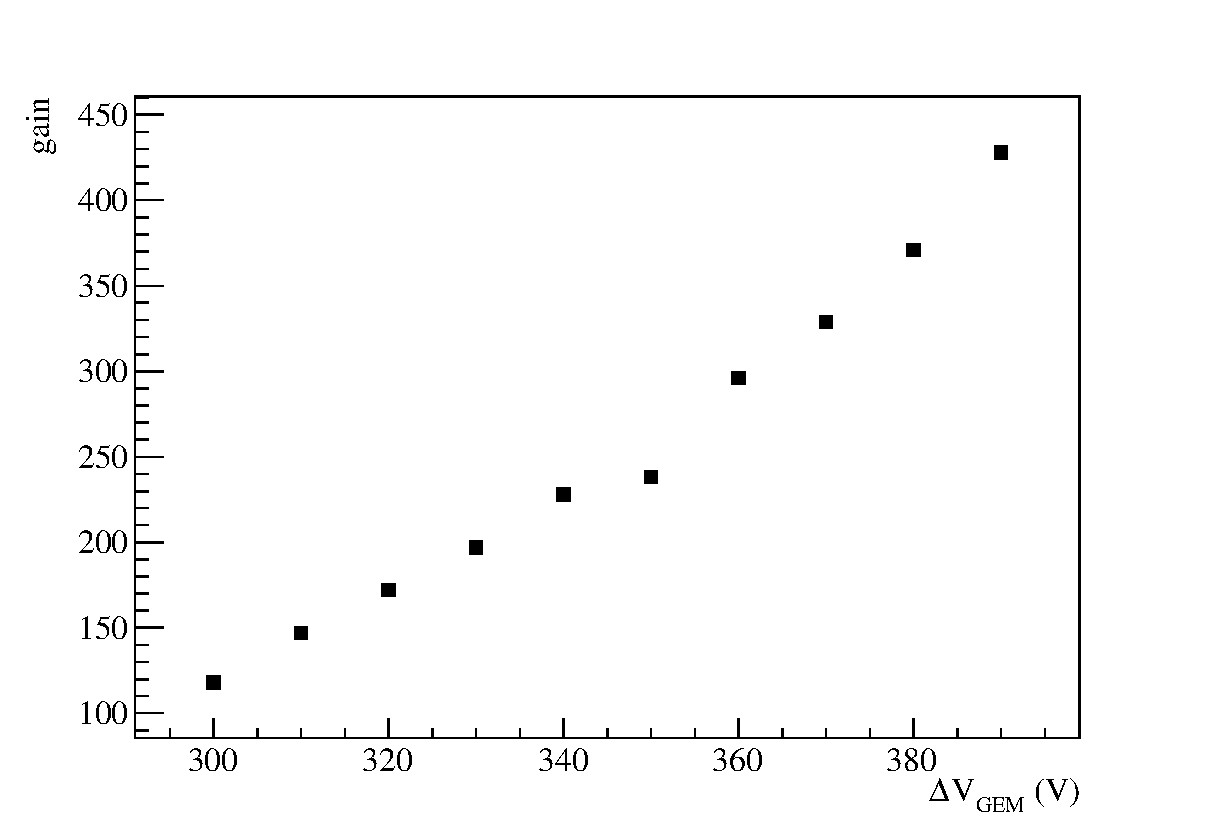
\includegraphics[clip, width=0.8\columnwidth]{gain_GEM_V_dep.eps}
  \scalebox{0.7}{\begin{tikzpicture}
\pgfdeclareplotmark{cross} {
\pgfpathmoveto{\pgfpoint{-0.3\pgfplotmarksize}{\pgfplotmarksize}}
\pgfpathlineto{\pgfpoint{+0.3\pgfplotmarksize}{\pgfplotmarksize}}
\pgfpathlineto{\pgfpoint{+0.3\pgfplotmarksize}{0.3\pgfplotmarksize}}
\pgfpathlineto{\pgfpoint{+1\pgfplotmarksize}{0.3\pgfplotmarksize}}
\pgfpathlineto{\pgfpoint{+1\pgfplotmarksize}{-0.3\pgfplotmarksize}}
\pgfpathlineto{\pgfpoint{+0.3\pgfplotmarksize}{-0.3\pgfplotmarksize}}
\pgfpathlineto{\pgfpoint{+0.3\pgfplotmarksize}{-1.\pgfplotmarksize}}
\pgfpathlineto{\pgfpoint{-0.3\pgfplotmarksize}{-1.\pgfplotmarksize}}
\pgfpathlineto{\pgfpoint{-0.3\pgfplotmarksize}{-0.3\pgfplotmarksize}}
\pgfpathlineto{\pgfpoint{-1.\pgfplotmarksize}{-0.3\pgfplotmarksize}}
\pgfpathlineto{\pgfpoint{-1.\pgfplotmarksize}{0.3\pgfplotmarksize}}
\pgfpathlineto{\pgfpoint{-0.3\pgfplotmarksize}{0.3\pgfplotmarksize}}
\pgfpathclose
\pgfusepathqstroke
}
\pgfdeclareplotmark{cross*} {
\pgfpathmoveto{\pgfpoint{-0.3\pgfplotmarksize}{\pgfplotmarksize}}
\pgfpathlineto{\pgfpoint{+0.3\pgfplotmarksize}{\pgfplotmarksize}}
\pgfpathlineto{\pgfpoint{+0.3\pgfplotmarksize}{0.3\pgfplotmarksize}}
\pgfpathlineto{\pgfpoint{+1\pgfplotmarksize}{0.3\pgfplotmarksize}}
\pgfpathlineto{\pgfpoint{+1\pgfplotmarksize}{-0.3\pgfplotmarksize}}
\pgfpathlineto{\pgfpoint{+0.3\pgfplotmarksize}{-0.3\pgfplotmarksize}}
\pgfpathlineto{\pgfpoint{+0.3\pgfplotmarksize}{-1.\pgfplotmarksize}}
\pgfpathlineto{\pgfpoint{-0.3\pgfplotmarksize}{-1.\pgfplotmarksize}}
\pgfpathlineto{\pgfpoint{-0.3\pgfplotmarksize}{-0.3\pgfplotmarksize}}
\pgfpathlineto{\pgfpoint{-1.\pgfplotmarksize}{-0.3\pgfplotmarksize}}
\pgfpathlineto{\pgfpoint{-1.\pgfplotmarksize}{0.3\pgfplotmarksize}}
\pgfpathlineto{\pgfpoint{-0.3\pgfplotmarksize}{0.3\pgfplotmarksize}}
\pgfpathclose
\pgfusepathqfillstroke
}
\pgfdeclareplotmark{newstar} {
\pgfpathmoveto{\pgfqpoint{0pt}{\pgfplotmarksize}}
\pgfpathlineto{\pgfqpointpolar{44}{0.5\pgfplotmarksize}}
\pgfpathlineto{\pgfqpointpolar{18}{\pgfplotmarksize}}
\pgfpathlineto{\pgfqpointpolar{-20}{0.5\pgfplotmarksize}}
\pgfpathlineto{\pgfqpointpolar{-54}{\pgfplotmarksize}}
\pgfpathlineto{\pgfqpointpolar{-90}{0.5\pgfplotmarksize}}
\pgfpathlineto{\pgfqpointpolar{234}{\pgfplotmarksize}}
\pgfpathlineto{\pgfqpointpolar{198}{0.5\pgfplotmarksize}}
\pgfpathlineto{\pgfqpointpolar{162}{\pgfplotmarksize}}
\pgfpathlineto{\pgfqpointpolar{134}{0.5\pgfplotmarksize}}
\pgfpathclose
\pgfusepathqstroke
}
\pgfdeclareplotmark{newstar*} {
\pgfpathmoveto{\pgfqpoint{0pt}{\pgfplotmarksize}}
\pgfpathlineto{\pgfqpointpolar{44}{0.5\pgfplotmarksize}}
\pgfpathlineto{\pgfqpointpolar{18}{\pgfplotmarksize}}
\pgfpathlineto{\pgfqpointpolar{-20}{0.5\pgfplotmarksize}}
\pgfpathlineto{\pgfqpointpolar{-54}{\pgfplotmarksize}}
\pgfpathlineto{\pgfqpointpolar{-90}{0.5\pgfplotmarksize}}
\pgfpathlineto{\pgfqpointpolar{234}{\pgfplotmarksize}}
\pgfpathlineto{\pgfqpointpolar{198}{0.5\pgfplotmarksize}}
\pgfpathlineto{\pgfqpointpolar{162}{\pgfplotmarksize}}
\pgfpathlineto{\pgfqpointpolar{134}{0.5\pgfplotmarksize}}
\pgfpathclose
\pgfusepathqfillstroke
}
\definecolor{c}{rgb}{1,1,1};
\draw [color=c, fill=c] (0,0) rectangle (20,13.5817);
\draw [color=c, fill=c] (2,1.35817) rectangle (18,12.2235);
\definecolor{c}{rgb}{0,0,0};
\draw [c,line width=0.9] (2,1.35817) -- (2,12.2235) -- (18,12.2235) -- (18,1.35817) -- (2,1.35817);
\draw [c,line width=0.9] (2,1.35817) -- (18,1.35817);
\draw [c,line width=0.9] (3.33333,1.68413) -- (3.33333,1.35817);
\draw [c,line width=0.9] (4.07407,1.52115) -- (4.07407,1.35817);
\draw [c,line width=0.9] (4.81482,1.52115) -- (4.81482,1.35817);
\draw [c,line width=0.9] (5.55556,1.52115) -- (5.55556,1.35817);
\draw [c,line width=0.9] (6.2963,1.68413) -- (6.2963,1.35817);
\draw [c,line width=0.9] (7.03704,1.52115) -- (7.03704,1.35817);
\draw [c,line width=0.9] (7.77778,1.52115) -- (7.77778,1.35817);
\draw [c,line width=0.9] (8.51852,1.52115) -- (8.51852,1.35817);
\draw [c,line width=0.9] (9.25926,1.68413) -- (9.25926,1.35817);
\draw [c,line width=0.9] (10,1.52115) -- (10,1.35817);
\draw [c,line width=0.9] (10.7407,1.52115) -- (10.7407,1.35817);
\draw [c,line width=0.9] (11.4815,1.52115) -- (11.4815,1.35817);
\draw [c,line width=0.9] (12.2222,1.68413) -- (12.2222,1.35817);
\draw [c,line width=0.9] (12.963,1.52115) -- (12.963,1.35817);
\draw [c,line width=0.9] (13.7037,1.52115) -- (13.7037,1.35817);
\draw [c,line width=0.9] (14.4444,1.52115) -- (14.4444,1.35817);
\draw [c,line width=0.9] (15.1852,1.68413) -- (15.1852,1.35817);
\draw [c,line width=0.9] (3.33333,1.68413) -- (3.33333,1.35817);
\draw [c,line width=0.9] (2.59259,1.52115) -- (2.59259,1.35817);
\draw [c,line width=0.9] (15.1852,1.68413) -- (15.1852,1.35817);
\draw [c,line width=0.9] (15.9259,1.52115) -- (15.9259,1.35817);
\draw [c,line width=0.9] (16.6667,1.52115) -- (16.6667,1.35817);
\draw [c,line width=0.9] (17.4074,1.52115) -- (17.4074,1.35817);
\draw [anchor=base] (3.33333,0.801318) node[scale=1.3364, color=c, rotate=0]{300};
\draw [anchor=base] (6.2963,0.801318) node[scale=1.3364, color=c, rotate=0]{320};
\draw [anchor=base] (9.25926,0.801318) node[scale=1.3364, color=c, rotate=0]{340};
\draw [anchor=base] (12.2222,0.801318) node[scale=1.3364, color=c, rotate=0]{360};
\draw [anchor=base] (15.1852,0.801318) node[scale=1.3364, color=c, rotate=0]{380};
\draw [anchor= east] (18,0.380287) node[scale=1.3364, color=c, rotate=0]{$\Delta V_{\text{GEM}}\text{ (V)}$};
\draw [c,line width=0.9] (2,1.35817) -- (2,12.2235);
\draw [c,line width=0.9] (2.48,1.77926) -- (2,1.77926);
\draw [c,line width=0.9] (2.24,2.06877) -- (2,2.06877);
\draw [c,line width=0.9] (2.24,2.35828) -- (2,2.35828);
\draw [c,line width=0.9] (2.24,2.64779) -- (2,2.64779);
\draw [c,line width=0.9] (2.24,2.9373) -- (2,2.9373);
\draw [c,line width=0.9] (2.48,3.22681) -- (2,3.22681);
\draw [c,line width=0.9] (2.24,3.51632) -- (2,3.51632);
\draw [c,line width=0.9] (2.24,3.80583) -- (2,3.80583);
\draw [c,line width=0.9] (2.24,4.09534) -- (2,4.09534);
\draw [c,line width=0.9] (2.24,4.38485) -- (2,4.38485);
\draw [c,line width=0.9] (2.48,4.67436) -- (2,4.67436);
\draw [c,line width=0.9] (2.24,4.96387) -- (2,4.96387);
\draw [c,line width=0.9] (2.24,5.25339) -- (2,5.25339);
\draw [c,line width=0.9] (2.24,5.5429) -- (2,5.5429);
\draw [c,line width=0.9] (2.24,5.83241) -- (2,5.83241);
\draw [c,line width=0.9] (2.48,6.12192) -- (2,6.12192);
\draw [c,line width=0.9] (2.24,6.41143) -- (2,6.41143);
\draw [c,line width=0.9] (2.24,6.70094) -- (2,6.70094);
\draw [c,line width=0.9] (2.24,6.99045) -- (2,6.99045);
\draw [c,line width=0.9] (2.24,7.27996) -- (2,7.27996);
\draw [c,line width=0.9] (2.48,7.56947) -- (2,7.56947);
\draw [c,line width=0.9] (2.24,7.85898) -- (2,7.85898);
\draw [c,line width=0.9] (2.24,8.14849) -- (2,8.14849);
\draw [c,line width=0.9] (2.24,8.438) -- (2,8.438);
\draw [c,line width=0.9] (2.24,8.72751) -- (2,8.72751);
\draw [c,line width=0.9] (2.48,9.01702) -- (2,9.01702);
\draw [c,line width=0.9] (2.24,9.30653) -- (2,9.30653);
\draw [c,line width=0.9] (2.24,9.59604) -- (2,9.59604);
\draw [c,line width=0.9] (2.24,9.88555) -- (2,9.88555);
\draw [c,line width=0.9] (2.24,10.1751) -- (2,10.1751);
\draw [c,line width=0.9] (2.48,10.4646) -- (2,10.4646);
\draw [c,line width=0.9] (2.24,10.7541) -- (2,10.7541);
\draw [c,line width=0.9] (2.24,11.0436) -- (2,11.0436);
\draw [c,line width=0.9] (2.24,11.3331) -- (2,11.3331);
\draw [c,line width=0.9] (2.24,11.6226) -- (2,11.6226);
\draw [c,line width=0.9] (2.48,11.9121) -- (2,11.9121);
\draw [c,line width=0.9] (2.48,1.77926) -- (2,1.77926);
\draw [c,line width=0.9] (2.24,1.48975) -- (2,1.48975);
\draw [c,line width=0.9] (2.48,11.9121) -- (2,11.9121);
\draw [c,line width=0.9] (2.24,12.2016) -- (2,12.2016);
\draw [anchor= east] (1.9,1.77926) node[scale=1.3364, color=c, rotate=0]{100};
\draw [anchor= east] (1.9,3.22681) node[scale=1.3364, color=c, rotate=0]{150};
\draw [anchor= east] (1.9,4.67436) node[scale=1.3364, color=c, rotate=0]{200};
\draw [anchor= east] (1.9,6.12192) node[scale=1.3364, color=c, rotate=0]{250};
\draw [anchor= east] (1.9,7.56947) node[scale=1.3364, color=c, rotate=0]{300};
\draw [anchor= east] (1.9,9.01702) node[scale=1.3364, color=c, rotate=0]{350};
\draw [anchor= east] (1.9,10.4646) node[scale=1.3364, color=c, rotate=0]{400};
\draw [anchor= east] (1.9,11.9121) node[scale=1.3364, color=c, rotate=0]{450};
\draw [anchor= east] (0.416,12.2235) node[scale=1.3364, color=c, rotate=90]{gain};
\foreach \P in {(3.33333,2.30038), (4.81482,3.13996), (6.2963,3.86373), (7.77778,4.58751), (9.25926,5.48499), (10.7407,5.7745), (12.2222,7.45367), (13.7037,8.40905), (15.1852,9.62499), (16.6667,11.2752)}{\draw[mark options={color=c,fill=c},mark
 size=2.402402pt,mark=square*] plot coordinates {\P};}
\definecolor{c}{rgb}{1,0,0};
\draw [c,line width=1.8] (2.08,2.18828) -- (2.24,2.22879) -- (2.4,2.27057) -- (2.56,2.31361) -- (2.72,2.35792) -- (2.88,2.4035) -- (3.04,2.45035) -- (3.2,2.49846) -- (3.36,2.54784) -- (3.52,2.59849) -- (3.68,2.65041) -- (3.84,2.70359) -- (4,2.75804)
 -- (4.16,2.81376) -- (4.32,2.87074) -- (4.48,2.929) -- (4.64,2.98852) -- (4.8,3.0493) -- (4.96,3.11136) -- (5.12,3.17468) -- (5.28,3.23927) -- (5.44,3.30513) -- (5.6,3.37225) -- (5.76,3.44065) -- (5.92,3.51031) -- (6.08,3.58123) -- (6.24,3.65343) --
 (6.4,3.72689) -- (6.56,3.80162) -- (6.72,3.87761) -- (6.88,3.95488) -- (7.04,4.03341) -- (7.2,4.11321) -- (7.36,4.19427) -- (7.52,4.27661) -- (7.68,4.36021) -- (7.84,4.44508) -- (8,4.53121) -- (8.16,4.61861) -- (8.32,4.70728) -- (8.48,4.79722) --
 (8.64,4.88843) -- (8.8,4.9809) -- (8.96,5.07464) -- (9.12,5.16965) -- (9.28,5.26592) -- (9.44,5.36346) -- (9.6,5.46227) -- (9.76,5.56235) -- (9.92,5.6637);
\draw [c,line width=1.8] (9.92,5.6637) -- (10.08,5.76631) -- (10.24,5.87019) -- (10.4,5.97533) -- (10.56,6.08175) -- (10.72,6.18943) -- (10.88,6.29838) -- (11.04,6.4086) -- (11.2,6.52008) -- (11.36,6.63283) -- (11.52,6.74685) -- (11.68,6.86213) --
 (11.84,6.97869) -- (12,7.09651) -- (12.16,7.2156) -- (12.32,7.33595) -- (12.48,7.45758) -- (12.64,7.58047) -- (12.8,7.70462) -- (12.96,7.83005) -- (13.12,7.95674) -- (13.28,8.0847) -- (13.44,8.21393) -- (13.6,8.34442) -- (13.76,8.47619) --
 (13.92,8.60921) -- (14.08,8.74351) -- (14.24,8.87908) -- (14.4,9.01591) -- (14.56,9.15401) -- (14.72,9.29337) -- (14.88,9.43401) -- (15.04,9.57591) -- (15.2,9.71908) -- (15.36,9.86351) -- (15.52,10.0092) -- (15.68,10.1562) -- (15.84,10.3044) --
 (16,10.4539) -- (16.16,10.6047) -- (16.32,10.7567) -- (16.48,10.9101) -- (16.64,11.0646) -- (16.8,11.2205) -- (16.96,11.3776) -- (17.12,11.536) -- (17.28,11.6956) -- (17.44,11.8565) -- (17.6,12.0187) -- (17.76,12.1821);
\definecolor{c}{rgb}{0,0,0};
\foreach \P in {(3.33333,2.30038), (4.81482,3.13996), (6.2963,3.86373), (7.77778,4.58751), (9.25926,5.48499), (10.7407,5.7745), (12.2222,7.45367), (13.7037,8.40905), (15.1852,9.62499), (16.6667,11.2752)}{\draw[mark options={color=c,fill=c},mark
 size=2.402402pt,mark=square*] plot coordinates {\P};}
\end{tikzpicture}
}
  \caption{電子増幅率の$\Delta V_{\text{GEM}}$依存性.}
  \label{fig::gain_GEM_V_dep}
\end{figure}
%$\Delta V_{\rm GEM}$に対して増幅率が単調に増加していることが分かる.
増幅率の変化は$\mathit{gain} = 0.0188\times{\Delta V_{\text{GEM}}}^2-0.67\times{\Delta V_{\text{GEM}}}+1340$と
表すことができる.
$\Delta V_{\text{GEM}}$を大きくして,GEMの穴の中に生成される電場を強くすることでより強く増幅されることが確認された.

%$\Delta V_{\rm GEM} = 350 {\rm V}$とそれ以外では測定するタイミングが2時間ほどずれている.
%そのため,図\ref{fig::gain_GEM_V_dep}で$V_{\text{GEM}} = 350 {\text{V}}$のみ不連続に変化している.

\subsection{GEMと$\mu$-PICとの電位差による電子の増幅率}
$\Delta V_{\text{GEM-}\mu\text{-PIC}}$によってGEM で増幅された電子の$\mu$-PICによる収集率が変化する.
$\Delta V_{\text{GEM-}\mu\text{-PIC}}$を\SI{50}{\volt}間隔で\SIrange{550}{750}{\volt}の範囲で変化させて計10点測定した.
電子の増幅率の$\Delta V_{\text{GEM-}\mu\text{-PIC}}$による変化を図\ref{fig::gain_GEM_uPIC_V_dep}に示す.
\begin{figure}
  \centering
  \scalebox{0.7}{\begin{tikzpicture}
\pgfdeclareplotmark{cross} {
\pgfpathmoveto{\pgfpoint{-0.3\pgfplotmarksize}{\pgfplotmarksize}}
\pgfpathlineto{\pgfpoint{+0.3\pgfplotmarksize}{\pgfplotmarksize}}
\pgfpathlineto{\pgfpoint{+0.3\pgfplotmarksize}{0.3\pgfplotmarksize}}
\pgfpathlineto{\pgfpoint{+1\pgfplotmarksize}{0.3\pgfplotmarksize}}
\pgfpathlineto{\pgfpoint{+1\pgfplotmarksize}{-0.3\pgfplotmarksize}}
\pgfpathlineto{\pgfpoint{+0.3\pgfplotmarksize}{-0.3\pgfplotmarksize}}
\pgfpathlineto{\pgfpoint{+0.3\pgfplotmarksize}{-1.\pgfplotmarksize}}
\pgfpathlineto{\pgfpoint{-0.3\pgfplotmarksize}{-1.\pgfplotmarksize}}
\pgfpathlineto{\pgfpoint{-0.3\pgfplotmarksize}{-0.3\pgfplotmarksize}}
\pgfpathlineto{\pgfpoint{-1.\pgfplotmarksize}{-0.3\pgfplotmarksize}}
\pgfpathlineto{\pgfpoint{-1.\pgfplotmarksize}{0.3\pgfplotmarksize}}
\pgfpathlineto{\pgfpoint{-0.3\pgfplotmarksize}{0.3\pgfplotmarksize}}
\pgfpathclose
\pgfusepathqstroke
}
\pgfdeclareplotmark{cross*} {
\pgfpathmoveto{\pgfpoint{-0.3\pgfplotmarksize}{\pgfplotmarksize}}
\pgfpathlineto{\pgfpoint{+0.3\pgfplotmarksize}{\pgfplotmarksize}}
\pgfpathlineto{\pgfpoint{+0.3\pgfplotmarksize}{0.3\pgfplotmarksize}}
\pgfpathlineto{\pgfpoint{+1\pgfplotmarksize}{0.3\pgfplotmarksize}}
\pgfpathlineto{\pgfpoint{+1\pgfplotmarksize}{-0.3\pgfplotmarksize}}
\pgfpathlineto{\pgfpoint{+0.3\pgfplotmarksize}{-0.3\pgfplotmarksize}}
\pgfpathlineto{\pgfpoint{+0.3\pgfplotmarksize}{-1.\pgfplotmarksize}}
\pgfpathlineto{\pgfpoint{-0.3\pgfplotmarksize}{-1.\pgfplotmarksize}}
\pgfpathlineto{\pgfpoint{-0.3\pgfplotmarksize}{-0.3\pgfplotmarksize}}
\pgfpathlineto{\pgfpoint{-1.\pgfplotmarksize}{-0.3\pgfplotmarksize}}
\pgfpathlineto{\pgfpoint{-1.\pgfplotmarksize}{0.3\pgfplotmarksize}}
\pgfpathlineto{\pgfpoint{-0.3\pgfplotmarksize}{0.3\pgfplotmarksize}}
\pgfpathclose
\pgfusepathqfillstroke
}
\pgfdeclareplotmark{newstar} {
\pgfpathmoveto{\pgfqpoint{0pt}{\pgfplotmarksize}}
\pgfpathlineto{\pgfqpointpolar{44}{0.5\pgfplotmarksize}}
\pgfpathlineto{\pgfqpointpolar{18}{\pgfplotmarksize}}
\pgfpathlineto{\pgfqpointpolar{-20}{0.5\pgfplotmarksize}}
\pgfpathlineto{\pgfqpointpolar{-54}{\pgfplotmarksize}}
\pgfpathlineto{\pgfqpointpolar{-90}{0.5\pgfplotmarksize}}
\pgfpathlineto{\pgfqpointpolar{234}{\pgfplotmarksize}}
\pgfpathlineto{\pgfqpointpolar{198}{0.5\pgfplotmarksize}}
\pgfpathlineto{\pgfqpointpolar{162}{\pgfplotmarksize}}
\pgfpathlineto{\pgfqpointpolar{134}{0.5\pgfplotmarksize}}
\pgfpathclose
\pgfusepathqstroke
}
\pgfdeclareplotmark{newstar*} {
\pgfpathmoveto{\pgfqpoint{0pt}{\pgfplotmarksize}}
\pgfpathlineto{\pgfqpointpolar{44}{0.5\pgfplotmarksize}}
\pgfpathlineto{\pgfqpointpolar{18}{\pgfplotmarksize}}
\pgfpathlineto{\pgfqpointpolar{-20}{0.5\pgfplotmarksize}}
\pgfpathlineto{\pgfqpointpolar{-54}{\pgfplotmarksize}}
\pgfpathlineto{\pgfqpointpolar{-90}{0.5\pgfplotmarksize}}
\pgfpathlineto{\pgfqpointpolar{234}{\pgfplotmarksize}}
\pgfpathlineto{\pgfqpointpolar{198}{0.5\pgfplotmarksize}}
\pgfpathlineto{\pgfqpointpolar{162}{\pgfplotmarksize}}
\pgfpathlineto{\pgfqpointpolar{134}{0.5\pgfplotmarksize}}
\pgfpathclose
\pgfusepathqfillstroke
}
\definecolor{c}{rgb}{1,1,1};
\draw [color=c, fill=c] (0,0) rectangle (20,13.5817);
\draw [color=c, fill=c] (2,1.35817) rectangle (18,12.2235);
\definecolor{c}{rgb}{0,0,0};
\draw [c,line width=0.9] (2,1.35817) -- (2,12.2235) -- (18,12.2235) -- (18,1.35817) -- (2,1.35817);
\draw [c,line width=0.9] (2,1.35817) -- (18,1.35817);
\draw [c,line width=0.9] (3.33333,1.68413) -- (3.33333,1.35817);
\draw [c,line width=0.9] (4,1.52115) -- (4,1.35817);
\draw [c,line width=0.9] (4.66667,1.52115) -- (4.66667,1.35817);
\draw [c,line width=0.9] (5.33333,1.52115) -- (5.33333,1.35817);
\draw [c,line width=0.9] (6,1.52115) -- (6,1.35817);
\draw [c,line width=0.9] (6.66667,1.68413) -- (6.66667,1.35817);
\draw [c,line width=0.9] (7.33333,1.52115) -- (7.33333,1.35817);
\draw [c,line width=0.9] (8,1.52115) -- (8,1.35817);
\draw [c,line width=0.9] (8.66667,1.52115) -- (8.66667,1.35817);
\draw [c,line width=0.9] (9.33333,1.52115) -- (9.33333,1.35817);
\draw [c,line width=0.9] (10,1.68413) -- (10,1.35817);
\draw [c,line width=0.9] (10.6667,1.52115) -- (10.6667,1.35817);
\draw [c,line width=0.9] (11.3333,1.52115) -- (11.3333,1.35817);
\draw [c,line width=0.9] (12,1.52115) -- (12,1.35817);
\draw [c,line width=0.9] (12.6667,1.52115) -- (12.6667,1.35817);
\draw [c,line width=0.9] (13.3333,1.68413) -- (13.3333,1.35817);
\draw [c,line width=0.9] (14,1.52115) -- (14,1.35817);
\draw [c,line width=0.9] (14.6667,1.52115) -- (14.6667,1.35817);
\draw [c,line width=0.9] (15.3333,1.52115) -- (15.3333,1.35817);
\draw [c,line width=0.9] (16,1.52115) -- (16,1.35817);
\draw [c,line width=0.9] (16.6667,1.68413) -- (16.6667,1.35817);
\draw [c,line width=0.9] (3.33333,1.68413) -- (3.33333,1.35817);
\draw [c,line width=0.9] (2.66667,1.52115) -- (2.66667,1.35817);
\draw [c,line width=0.9] (2,1.52115) -- (2,1.35817);
\draw [c,line width=0.9] (16.6667,1.68413) -- (16.6667,1.35817);
\draw [c,line width=0.9] (17.3333,1.52115) -- (17.3333,1.35817);
\draw [anchor=base] (3.33333,0.801318) node[scale=1.3364, color=c, rotate=0]{550};
\draw [anchor=base] (6.66667,0.801318) node[scale=1.3364, color=c, rotate=0]{600};
\draw [anchor=base] (10,0.801318) node[scale=1.3364, color=c, rotate=0]{650};
\draw [anchor=base] (13.3333,0.801318) node[scale=1.3364, color=c, rotate=0]{700};
\draw [anchor=base] (16.6667,0.801318) node[scale=1.3364, color=c, rotate=0]{750};
\draw [anchor= east] (18,0.380287) node[scale=1.3364, color=c, rotate=0]{$\Delta V_{\text{GEM}-\mu\text{-PIC}}\text{ (V)}$};
\draw [c,line width=0.9] (2,1.35817) -- (2,12.2235);
\draw [c,line width=0.9] (2.48,1.73975) -- (2,1.73975);
\draw [c,line width=0.9] (2.24,2.02784) -- (2,2.02784);
\draw [c,line width=0.9] (2.24,2.31593) -- (2,2.31593);
\draw [c,line width=0.9] (2.24,2.60401) -- (2,2.60401);
\draw [c,line width=0.9] (2.48,2.8921) -- (2,2.8921);
\draw [c,line width=0.9] (2.24,3.18019) -- (2,3.18019);
\draw [c,line width=0.9] (2.24,3.46827) -- (2,3.46827);
\draw [c,line width=0.9] (2.24,3.75636) -- (2,3.75636);
\draw [c,line width=0.9] (2.48,4.04445) -- (2,4.04445);
\draw [c,line width=0.9] (2.24,4.33253) -- (2,4.33253);
\draw [c,line width=0.9] (2.24,4.62062) -- (2,4.62062);
\draw [c,line width=0.9] (2.24,4.9087) -- (2,4.9087);
\draw [c,line width=0.9] (2.48,5.19679) -- (2,5.19679);
\draw [c,line width=0.9] (2.24,5.48488) -- (2,5.48488);
\draw [c,line width=0.9] (2.24,5.77296) -- (2,5.77296);
\draw [c,line width=0.9] (2.24,6.06105) -- (2,6.06105);
\draw [c,line width=0.9] (2.48,6.34914) -- (2,6.34914);
\draw [c,line width=0.9] (2.24,6.63722) -- (2,6.63722);
\draw [c,line width=0.9] (2.24,6.92531) -- (2,6.92531);
\draw [c,line width=0.9] (2.24,7.2134) -- (2,7.2134);
\draw [c,line width=0.9] (2.48,7.50148) -- (2,7.50148);
\draw [c,line width=0.9] (2.24,7.78957) -- (2,7.78957);
\draw [c,line width=0.9] (2.24,8.07766) -- (2,8.07766);
\draw [c,line width=0.9] (2.24,8.36574) -- (2,8.36574);
\draw [c,line width=0.9] (2.48,8.65383) -- (2,8.65383);
\draw [c,line width=0.9] (2.24,8.94191) -- (2,8.94191);
\draw [c,line width=0.9] (2.24,9.23) -- (2,9.23);
\draw [c,line width=0.9] (2.24,9.51809) -- (2,9.51809);
\draw [c,line width=0.9] (2.48,9.80617) -- (2,9.80617);
\draw [c,line width=0.9] (2.24,10.0943) -- (2,10.0943);
\draw [c,line width=0.9] (2.24,10.3823) -- (2,10.3823);
\draw [c,line width=0.9] (2.24,10.6704) -- (2,10.6704);
\draw [c,line width=0.9] (2.48,10.9585) -- (2,10.9585);
\draw [c,line width=0.9] (2.24,11.2466) -- (2,11.2466);
\draw [c,line width=0.9] (2.24,11.5347) -- (2,11.5347);
\draw [c,line width=0.9] (2.24,11.8228) -- (2,11.8228);
\draw [c,line width=0.9] (2.48,12.1109) -- (2,12.1109);
\draw [c,line width=0.9] (2.48,1.73975) -- (2,1.73975);
\draw [c,line width=0.9] (2.24,1.45167) -- (2,1.45167);
\draw [c,line width=0.9] (2.48,12.1109) -- (2,12.1109);
\draw [anchor= east] (1.9,1.73975) node[scale=1.3364, color=c, rotate=0]{160};
\draw [anchor= east] (1.9,2.8921) node[scale=1.3364, color=c, rotate=0]{180};
\draw [anchor= east] (1.9,4.04445) node[scale=1.3364, color=c, rotate=0]{200};
\draw [anchor= east] (1.9,5.19679) node[scale=1.3364, color=c, rotate=0]{220};
\draw [anchor= east] (1.9,6.34914) node[scale=1.3364, color=c, rotate=0]{240};
\draw [anchor= east] (1.9,7.50148) node[scale=1.3364, color=c, rotate=0]{260};
\draw [anchor= east] (1.9,8.65383) node[scale=1.3364, color=c, rotate=0]{280};
\draw [anchor= east] (1.9,9.80617) node[scale=1.3364, color=c, rotate=0]{300};
\draw [anchor= east] (1.9,10.9585) node[scale=1.3364, color=c, rotate=0]{320};
\draw [anchor= east] (1.9,12.1109) node[scale=1.3364, color=c, rotate=0]{340};
\draw [anchor= east] (0.416,12.2235) node[scale=1.3364, color=c, rotate=90]{gain};
\foreach \P in {(3.33333,2.31593), (6.66667,4.67824), (10,6.2339), (13.3333,9.11477), (16.6667,11.2466)}{\draw[mark options={color=c,fill=c},mark size=2.402402pt,mark=square*] plot coordinates {\P};}
\end{tikzpicture}
}
  \caption{電子増幅率の$\Delta V_{\text{GEM-}\mu\text{-PIC}}$依存性.}
  \label{fig::gain_GEM_uPIC_V_dep}
\end{figure}
増幅率の変化は$\mathit{gain} = 0.767\times{\Delta V_{\text{GEM-}\mu\text{-PIC}}}$と
表すことができる.
GEMで増幅された電子をより強い電場で移動させることで,効率よく$\mu$-PICに電子が輸送されたと考えられる.

\subsection{$\mu$-PICによる電子増幅率}
電子は$\mu$-PICで読み出される直前に,$\mu$-PICによって作られた高電場によって増幅される.
$V_{\mu\text{-PIC}}$を\SI{10}{\volt}間隔で\SIrange{350}{440}{\volt}の範囲で変化させて計10点測定した.
電子の増幅率の$V_{\mu\text{-PIC}}$ による変化を図\ref{fig::gain_uPIC_V_dep}に示す.
\begin{figure}
  \centering
%  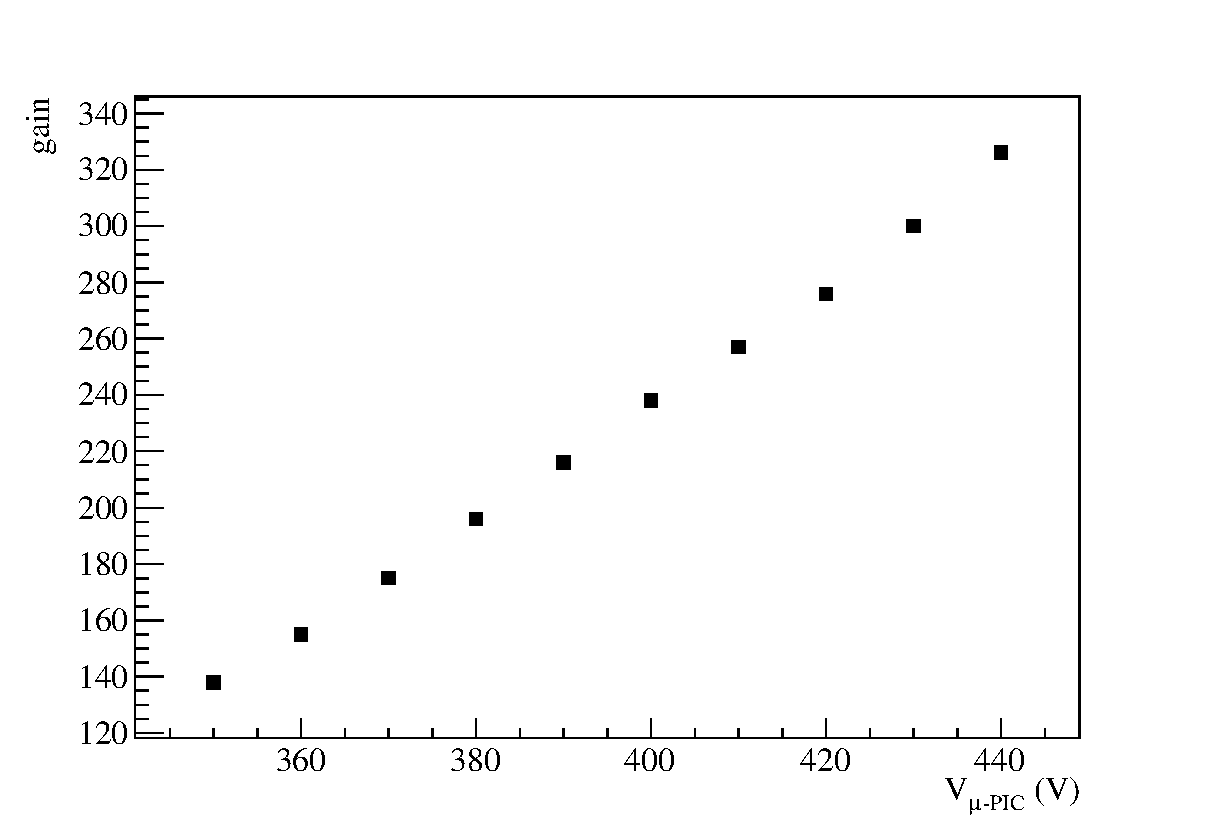
\includegraphics[clip, width=0.8\columnwidth]{gain_uPIC_V_dep.eps}
  \scalebox{0.7}{\begin{tikzpicture}
\pgfdeclareplotmark{cross} {
\pgfpathmoveto{\pgfpoint{-0.3\pgfplotmarksize}{\pgfplotmarksize}}
\pgfpathlineto{\pgfpoint{+0.3\pgfplotmarksize}{\pgfplotmarksize}}
\pgfpathlineto{\pgfpoint{+0.3\pgfplotmarksize}{0.3\pgfplotmarksize}}
\pgfpathlineto{\pgfpoint{+1\pgfplotmarksize}{0.3\pgfplotmarksize}}
\pgfpathlineto{\pgfpoint{+1\pgfplotmarksize}{-0.3\pgfplotmarksize}}
\pgfpathlineto{\pgfpoint{+0.3\pgfplotmarksize}{-0.3\pgfplotmarksize}}
\pgfpathlineto{\pgfpoint{+0.3\pgfplotmarksize}{-1.\pgfplotmarksize}}
\pgfpathlineto{\pgfpoint{-0.3\pgfplotmarksize}{-1.\pgfplotmarksize}}
\pgfpathlineto{\pgfpoint{-0.3\pgfplotmarksize}{-0.3\pgfplotmarksize}}
\pgfpathlineto{\pgfpoint{-1.\pgfplotmarksize}{-0.3\pgfplotmarksize}}
\pgfpathlineto{\pgfpoint{-1.\pgfplotmarksize}{0.3\pgfplotmarksize}}
\pgfpathlineto{\pgfpoint{-0.3\pgfplotmarksize}{0.3\pgfplotmarksize}}
\pgfpathclose
\pgfusepathqstroke
}
\pgfdeclareplotmark{cross*} {
\pgfpathmoveto{\pgfpoint{-0.3\pgfplotmarksize}{\pgfplotmarksize}}
\pgfpathlineto{\pgfpoint{+0.3\pgfplotmarksize}{\pgfplotmarksize}}
\pgfpathlineto{\pgfpoint{+0.3\pgfplotmarksize}{0.3\pgfplotmarksize}}
\pgfpathlineto{\pgfpoint{+1\pgfplotmarksize}{0.3\pgfplotmarksize}}
\pgfpathlineto{\pgfpoint{+1\pgfplotmarksize}{-0.3\pgfplotmarksize}}
\pgfpathlineto{\pgfpoint{+0.3\pgfplotmarksize}{-0.3\pgfplotmarksize}}
\pgfpathlineto{\pgfpoint{+0.3\pgfplotmarksize}{-1.\pgfplotmarksize}}
\pgfpathlineto{\pgfpoint{-0.3\pgfplotmarksize}{-1.\pgfplotmarksize}}
\pgfpathlineto{\pgfpoint{-0.3\pgfplotmarksize}{-0.3\pgfplotmarksize}}
\pgfpathlineto{\pgfpoint{-1.\pgfplotmarksize}{-0.3\pgfplotmarksize}}
\pgfpathlineto{\pgfpoint{-1.\pgfplotmarksize}{0.3\pgfplotmarksize}}
\pgfpathlineto{\pgfpoint{-0.3\pgfplotmarksize}{0.3\pgfplotmarksize}}
\pgfpathclose
\pgfusepathqfillstroke
}
\pgfdeclareplotmark{newstar} {
\pgfpathmoveto{\pgfqpoint{0pt}{\pgfplotmarksize}}
\pgfpathlineto{\pgfqpointpolar{44}{0.5\pgfplotmarksize}}
\pgfpathlineto{\pgfqpointpolar{18}{\pgfplotmarksize}}
\pgfpathlineto{\pgfqpointpolar{-20}{0.5\pgfplotmarksize}}
\pgfpathlineto{\pgfqpointpolar{-54}{\pgfplotmarksize}}
\pgfpathlineto{\pgfqpointpolar{-90}{0.5\pgfplotmarksize}}
\pgfpathlineto{\pgfqpointpolar{234}{\pgfplotmarksize}}
\pgfpathlineto{\pgfqpointpolar{198}{0.5\pgfplotmarksize}}
\pgfpathlineto{\pgfqpointpolar{162}{\pgfplotmarksize}}
\pgfpathlineto{\pgfqpointpolar{134}{0.5\pgfplotmarksize}}
\pgfpathclose
\pgfusepathqstroke
}
\pgfdeclareplotmark{newstar*} {
\pgfpathmoveto{\pgfqpoint{0pt}{\pgfplotmarksize}}
\pgfpathlineto{\pgfqpointpolar{44}{0.5\pgfplotmarksize}}
\pgfpathlineto{\pgfqpointpolar{18}{\pgfplotmarksize}}
\pgfpathlineto{\pgfqpointpolar{-20}{0.5\pgfplotmarksize}}
\pgfpathlineto{\pgfqpointpolar{-54}{\pgfplotmarksize}}
\pgfpathlineto{\pgfqpointpolar{-90}{0.5\pgfplotmarksize}}
\pgfpathlineto{\pgfqpointpolar{234}{\pgfplotmarksize}}
\pgfpathlineto{\pgfqpointpolar{198}{0.5\pgfplotmarksize}}
\pgfpathlineto{\pgfqpointpolar{162}{\pgfplotmarksize}}
\pgfpathlineto{\pgfqpointpolar{134}{0.5\pgfplotmarksize}}
\pgfpathclose
\pgfusepathqfillstroke
}
\definecolor{c}{rgb}{1,1,1};
\draw [color=c, fill=c] (0,0) rectangle (20,13.5817);
\draw [color=c, fill=c] (2,1.35817) rectangle (18,12.2235);
\definecolor{c}{rgb}{0,0,0};
\draw [c,line width=0.9] (2,1.35817) -- (2,12.2235) -- (18,12.2235) -- (18,1.35817) -- (2,1.35817);
\draw [c,line width=0.9] (2,1.35817) -- (18,1.35817);
\draw [c,line width=0.9] (4.81482,1.68413) -- (4.81482,1.35817);
\draw [c,line width=0.9] (5.55556,1.52115) -- (5.55556,1.35817);
\draw [c,line width=0.9] (6.2963,1.52115) -- (6.2963,1.35817);
\draw [c,line width=0.9] (7.03704,1.52115) -- (7.03704,1.35817);
\draw [c,line width=0.9] (7.77778,1.68413) -- (7.77778,1.35817);
\draw [c,line width=0.9] (8.51852,1.52115) -- (8.51852,1.35817);
\draw [c,line width=0.9] (9.25926,1.52115) -- (9.25926,1.35817);
\draw [c,line width=0.9] (10,1.52115) -- (10,1.35817);
\draw [c,line width=0.9] (10.7407,1.68413) -- (10.7407,1.35817);
\draw [c,line width=0.9] (11.4815,1.52115) -- (11.4815,1.35817);
\draw [c,line width=0.9] (12.2222,1.52115) -- (12.2222,1.35817);
\draw [c,line width=0.9] (12.963,1.52115) -- (12.963,1.35817);
\draw [c,line width=0.9] (13.7037,1.68413) -- (13.7037,1.35817);
\draw [c,line width=0.9] (14.4444,1.52115) -- (14.4444,1.35817);
\draw [c,line width=0.9] (15.1852,1.52115) -- (15.1852,1.35817);
\draw [c,line width=0.9] (15.9259,1.52115) -- (15.9259,1.35817);
\draw [c,line width=0.9] (16.6667,1.68413) -- (16.6667,1.35817);
\draw [c,line width=0.9] (4.81482,1.68413) -- (4.81482,1.35817);
\draw [c,line width=0.9] (4.07407,1.52115) -- (4.07407,1.35817);
\draw [c,line width=0.9] (3.33333,1.52115) -- (3.33333,1.35817);
\draw [c,line width=0.9] (2.59259,1.52115) -- (2.59259,1.35817);
\draw [c,line width=0.9] (16.6667,1.68413) -- (16.6667,1.35817);
\draw [c,line width=0.9] (17.4074,1.52115) -- (17.4074,1.35817);
\draw [anchor=base] (4.81482,0.801318) node[scale=1.3364, color=c, rotate=0]{360};
\draw [anchor=base] (7.77778,0.801318) node[scale=1.3364, color=c, rotate=0]{380};
\draw [anchor=base] (10.7407,0.801318) node[scale=1.3364, color=c, rotate=0]{400};
\draw [anchor=base] (13.7037,0.801318) node[scale=1.3364, color=c, rotate=0]{420};
\draw [anchor=base] (16.6667,0.801318) node[scale=1.3364, color=c, rotate=0]{440};
\draw [anchor= east] (18,0.380287) node[scale=1.3364, color=c, rotate=0]{$V_{\mu\text{-PIC}}\text{ (V)}$};
\draw [c,line width=0.9] (2,1.35817) -- (2,12.2235);
\draw [c,line width=0.9] (2.48,1.44571) -- (2,1.44571);
\draw [c,line width=0.9] (2.24,1.68414) -- (2,1.68414);
\draw [c,line width=0.9] (2.24,1.92256) -- (2,1.92256);
\draw [c,line width=0.9] (2.24,2.16099) -- (2,2.16099);
\draw [c,line width=0.9] (2.48,2.39942) -- (2,2.39942);
\draw [c,line width=0.9] (2.24,2.63785) -- (2,2.63785);
\draw [c,line width=0.9] (2.24,2.87627) -- (2,2.87627);
\draw [c,line width=0.9] (2.24,3.1147) -- (2,3.1147);
\draw [c,line width=0.9] (2.48,3.35313) -- (2,3.35313);
\draw [c,line width=0.9] (2.24,3.59156) -- (2,3.59156);
\draw [c,line width=0.9] (2.24,3.82999) -- (2,3.82999);
\draw [c,line width=0.9] (2.24,4.06841) -- (2,4.06841);
\draw [c,line width=0.9] (2.48,4.30684) -- (2,4.30684);
\draw [c,line width=0.9] (2.24,4.54527) -- (2,4.54527);
\draw [c,line width=0.9] (2.24,4.7837) -- (2,4.7837);
\draw [c,line width=0.9] (2.24,5.02213) -- (2,5.02213);
\draw [c,line width=0.9] (2.48,5.26055) -- (2,5.26055);
\draw [c,line width=0.9] (2.24,5.49898) -- (2,5.49898);
\draw [c,line width=0.9] (2.24,5.73741) -- (2,5.73741);
\draw [c,line width=0.9] (2.24,5.97584) -- (2,5.97584);
\draw [c,line width=0.9] (2.48,6.21426) -- (2,6.21426);
\draw [c,line width=0.9] (2.24,6.45269) -- (2,6.45269);
\draw [c,line width=0.9] (2.24,6.69112) -- (2,6.69112);
\draw [c,line width=0.9] (2.24,6.92955) -- (2,6.92955);
\draw [c,line width=0.9] (2.48,7.16798) -- (2,7.16798);
\draw [c,line width=0.9] (2.24,7.4064) -- (2,7.4064);
\draw [c,line width=0.9] (2.24,7.64483) -- (2,7.64483);
\draw [c,line width=0.9] (2.24,7.88326) -- (2,7.88326);
\draw [c,line width=0.9] (2.48,8.12169) -- (2,8.12169);
\draw [c,line width=0.9] (2.24,8.36012) -- (2,8.36012);
\draw [c,line width=0.9] (2.24,8.59854) -- (2,8.59854);
\draw [c,line width=0.9] (2.24,8.83697) -- (2,8.83697);
\draw [c,line width=0.9] (2.48,9.0754) -- (2,9.0754);
\draw [c,line width=0.9] (2.24,9.31383) -- (2,9.31383);
\draw [c,line width=0.9] (2.24,9.55225) -- (2,9.55225);
\draw [c,line width=0.9] (2.24,9.79068) -- (2,9.79068);
\draw [c,line width=0.9] (2.48,10.0291) -- (2,10.0291);
\draw [c,line width=0.9] (2.24,10.2675) -- (2,10.2675);
\draw [c,line width=0.9] (2.24,10.506) -- (2,10.506);
\draw [c,line width=0.9] (2.24,10.7444) -- (2,10.7444);
\draw [c,line width=0.9] (2.48,10.9828) -- (2,10.9828);
\draw [c,line width=0.9] (2.24,11.2212) -- (2,11.2212);
\draw [c,line width=0.9] (2.24,11.4597) -- (2,11.4597);
\draw [c,line width=0.9] (2.24,11.6981) -- (2,11.6981);
\draw [c,line width=0.9] (2.48,11.9365) -- (2,11.9365);
\draw [c,line width=0.9] (2.48,1.44571) -- (2,1.44571);
\draw [c,line width=0.9] (2.48,11.9365) -- (2,11.9365);
\draw [c,line width=0.9] (2.24,12.175) -- (2,12.175);
\draw [anchor= east] (1.9,1.44571) node[scale=1.3364, color=c, rotate=0]{120};
\draw [anchor= east] (1.9,2.39942) node[scale=1.3364, color=c, rotate=0]{140};
\draw [anchor= east] (1.9,3.35313) node[scale=1.3364, color=c, rotate=0]{160};
\draw [anchor= east] (1.9,4.30684) node[scale=1.3364, color=c, rotate=0]{180};
\draw [anchor= east] (1.9,5.26055) node[scale=1.3364, color=c, rotate=0]{200};
\draw [anchor= east] (1.9,6.21426) node[scale=1.3364, color=c, rotate=0]{220};
\draw [anchor= east] (1.9,7.16798) node[scale=1.3364, color=c, rotate=0]{240};
\draw [anchor= east] (1.9,8.12169) node[scale=1.3364, color=c, rotate=0]{260};
\draw [anchor= east] (1.9,9.0754) node[scale=1.3364, color=c, rotate=0]{280};
\draw [anchor= east] (1.9,10.0291) node[scale=1.3364, color=c, rotate=0]{300};
\draw [anchor= east] (1.9,10.9828) node[scale=1.3364, color=c, rotate=0]{320};
\draw [anchor= east] (1.9,11.9365) node[scale=1.3364, color=c, rotate=0]{340};
\draw [anchor= east] (0.416,12.2235) node[scale=1.3364, color=c, rotate=90]{gain};
\foreach \P in {(16.6667,11.2689), (15.1852,10.0291), (13.7037,8.88466), (12.2222,7.97863), (10.7407,7.07261), (9.25926,6.02352), (7.77778,5.06981), (6.2963,4.06841), (4.81482,3.1147), (3.33333,2.30405)}{\draw[mark options={color=c,fill=c},mark
 size=2.402402pt,mark=square*] plot coordinates {\P};}
\end{tikzpicture}
}
  \caption{電子増幅率の$V_{\mu\text{-PIC}}$依存性.}
  \label{fig::gain_uPIC_V_dep}
\end{figure}
%$V_{\rm\mu-PIC}$に対して増幅率が単調に増加していることが分かる.
増幅率の変化は$\mathit{gain} = 2.06\times{V_{\mu\text{-PIC}}}-253$と表すことができる.
$\mu$-PICのanode 電極の周りにより強い電場が形成されることで,より強く電子が増幅されることが確認された.
%GEMによる増幅率と異なり,$\mu$-PICの電圧依存性はほぼ同時に測定したため,
%図\ref{fig::gain_GEM_V_dep}に見られたような不連続性は見られない.

\section{電子のディフュージョン効果}
ドリフトスピードが一定である場合は,電子の拡散は$\sqrt{L}$に比例する.
線源は線源導入機によって,チェンバーの気密性を保持したまま電子のドリフト方向に移動可能である.
線源導入機は2016年度の森本修論~\cite{morimoto_thesis}で開発された.
図\ref{pic::source_insirtion}に線源導入機の先に線源を取り付けた様子を示す.
図\ref{pic::source_insirtion}中の矢印の方向に線源を移動させることができる.
\begin{figure}
  \centering
  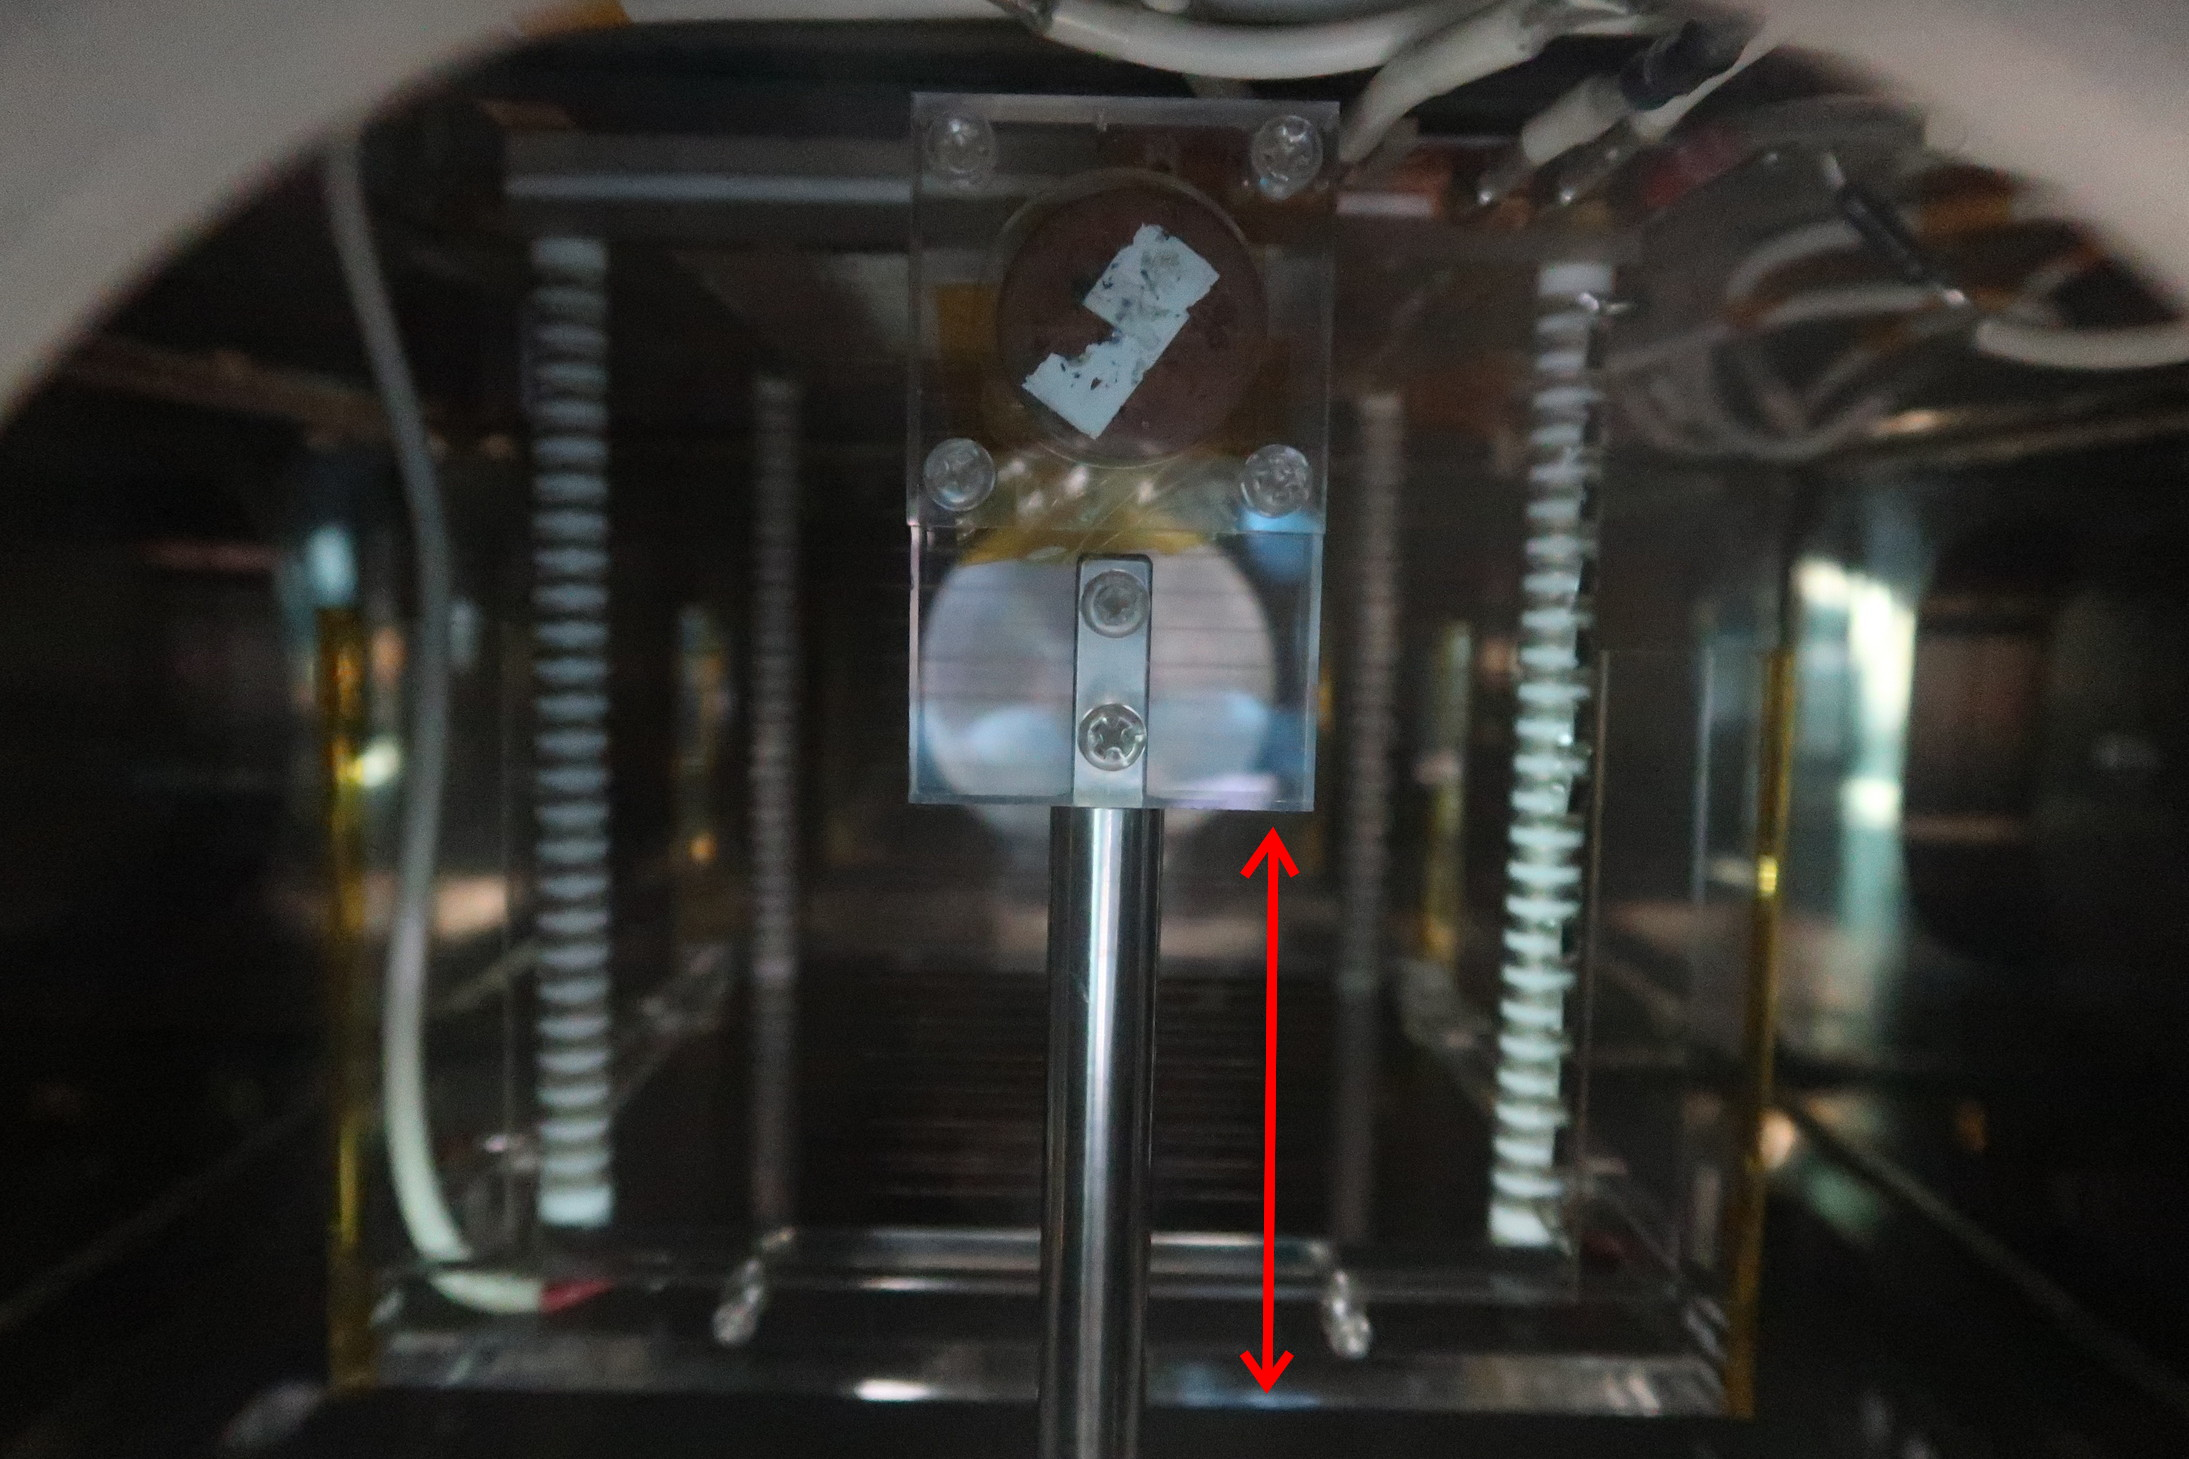
\includegraphics[clip, width=0.8\columnwidth]{IMG_2923_drawed.jpg}
  \caption[線源導入機に取り付けたれた線源.]
          {線源導入機に取り付けたれた線源.
          矢印の方向に移動させることができる.}
  \label{pic::source_insirtion}
\end{figure}
線源導入機によって線源の位置を変化させることで,拡散効果の$L$依存性を調べることができる.
拡散効果とトラックの太さが比例していると仮定すると,track width $\sim\sqrt{L}$にとなる.
トラックの太さと線源の位置との依存性を図\ref{fig::diff_x}に示す.
図\ref{fig::diff_x}の$L$は線源コリメータの\ang{0}穴とgridとのドリフト方向の距離である.
\begin{figure}
  \centering
  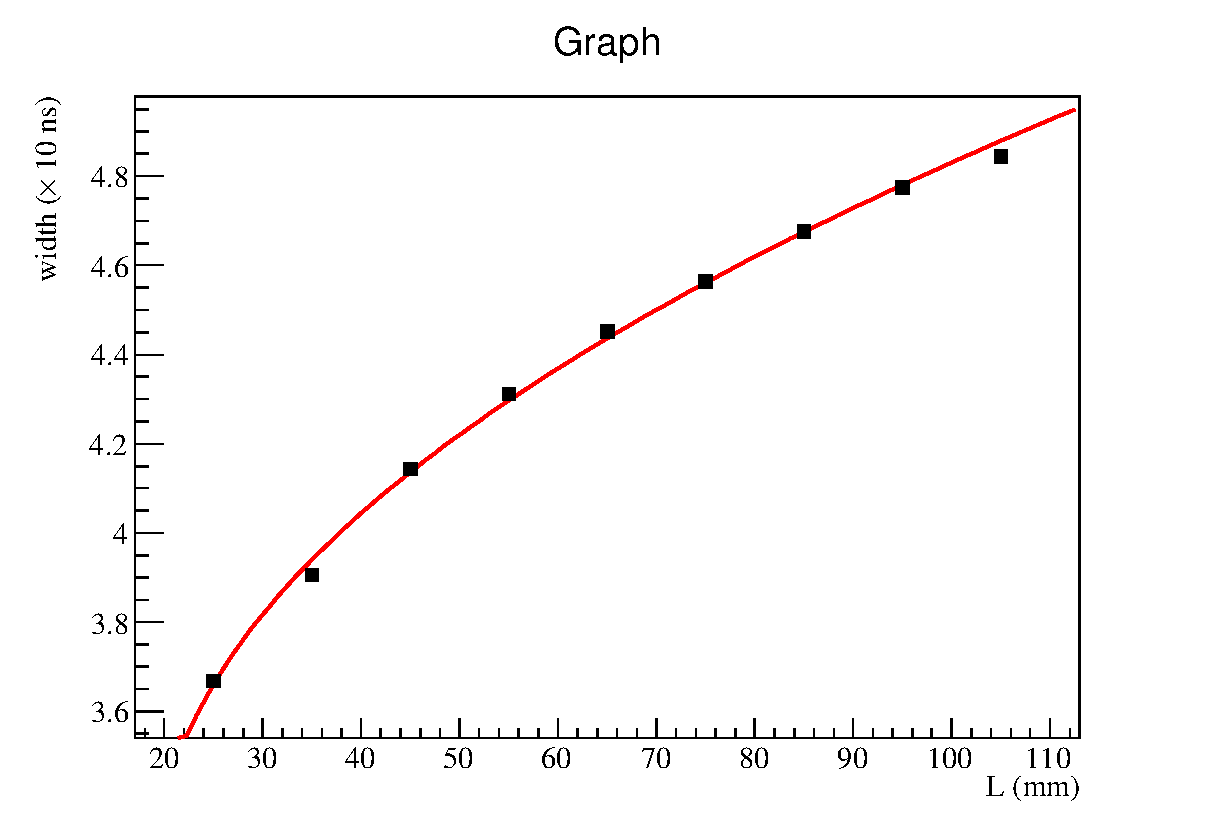
\includegraphics[clip, width=0.8\columnwidth]{diff_x.eps}
  \caption{トラックの太さの位置依存性.}
  \label{fig::diff_x}
\end{figure}
$\text{track width} = 1.27\times\sqrt{L-19.2}+23.1$となり,
$\sqrt{L}$に比例していることが確認された.

%\subsection{ドリフトスピードの時間安定性}
%低圧では露点などの不純物が混ざることによって、ドリフトスピードが変化することが懸念される。
%そこで、ドリフトスピードの時間安定性の測定を行った。
%この測定は$\rm CH_{4}$ 50 hPa で行った。

\section{検出効率}
測定されたトラックの長さから粒子のエネルギーを決定する.
しかし,散乱点や粒子の運動エネルギー,角度によってはMAIKo TPC の有感領域から外に出てしまう.
有感領域の外へ出てしまった粒子のトラックの長さは決定することができないので,
その粒子の運動エネルギーと運動量を決定できなくなってしまう.
そこで,有感領域内で停止する割合(検出効率)を考える.

ここでは,以下のようなで状況を考える.
\begin{itemize}
\item
  半径\SI{10}{\milli\metre}の\SI{14}{\mega\electronvolt}の中性子ビームが$z$軸正の向きでMAIKo TPC に入射している.
\item
  ビーム軸方向に一様に中性子と${}^{12}\mathrm{C}$の散乱が起きる.
\item
  散乱の角度分布は図\ref{fig::sig_angle_dist}とする.
\end{itemize}
半径\SI{10}{\milli\metre}の幅を持っている中性子ビームを用いると,
散乱点が$y$軸方向に\SI{20}{\milli\metre}の幅を持つ.
gridの座標を$y = \SI{0}{\milli\metre}$,plateの座標を$y = \SI{140}{\milli\metre}$とし,
ビームの中心が$y = \SI{70}{\milli\metre}$の位置にあるとする.
この時$y = \SI{80}{\milli\metre}$の位置で散乱が起きると,
見かけ上の有感領域はgrid方向に\SI{80}{\milli\metre},plate方向に\SI{60}{\milli\metre}となる.
また,$y = \SI{60}{\milli\metre}$の位置で散乱が起きると,
見かけ上の有感領域はgrid方向に\SI{60}{\milli\metre},plate方向に\SI{80}{\milli\metre}となる.
しかし,MAIKo TPC は$y$座標をトラックの周囲に発生した電子の読み出し面に到達する時間差を用いて検出しているため,
$y$座標の絶対値を決定することができない.
すると,$y = \SI{80}{\milli\metre}$と$y = \SI{60}{\milli\metre}$のどちらで散乱が起きたのかを区別できない.
どちらの場合でも確実に有感領域中で停止したと保証するためには,
散乱点から$y$軸方向に\SI{\pm60}{\milli\metre}を実質の有感領域としなければならない.

この条件のもとで,散乱点および3つの停止点が有感領域にある時に検出可能とする.
すると検出効率は\SI{48.2}{\percent}となった.
検出効率の散乱点の$z$座標依存性を図\ref{fig::detection_efficiency_beam_axis}に,
${}^{12}\mathrm{C}$の重心系での散乱角依存性を図\ref{fig::detection_efficiency_theta_cm}に示す.
図\ref{fig::detection_efficiency_beam_axis}から分かるように,
$z$座標が小さいまたは大きい場所で反応が起きた場合に,
崩壊してできた$\alpha$粒子が有感領域から出やすくなるため検出効率が低下している.
また,図\ref{fig::detection_efficiency_theta_cm}から分かるように,
$\theta_{\text{c.m.}}$が小さいところで検出効率が低下している.
これは,$\theta_{\text{c.m.}}$が小さいところでは中性子から多くのエネルギーを受け取り,
崩壊した$\alpha$粒子が全体的に$z$軸正の方向にブーストされることで有感領域から出ていきやすくなるためである.

\begin{figure}
  \centering
  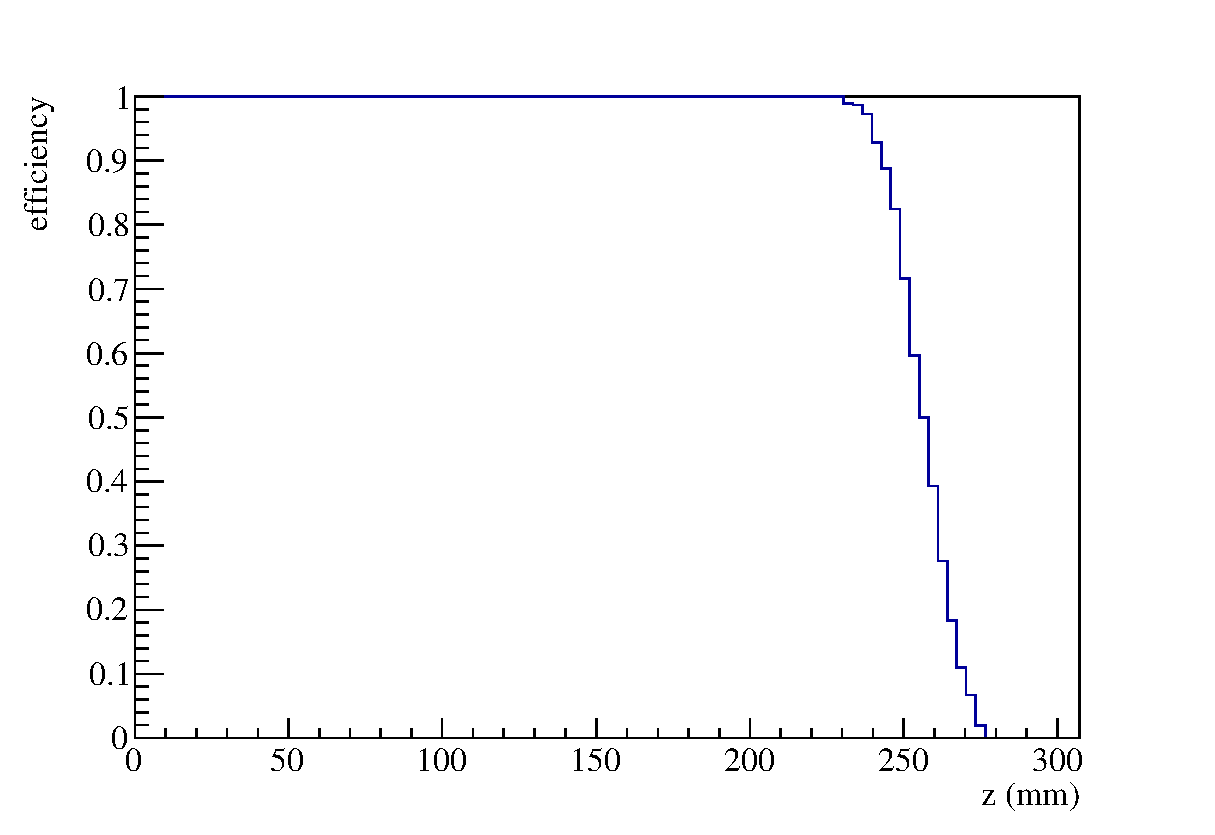
\includegraphics[clip, width=0.8\columnwidth]{detection_efficiency_beam_axis.eps}
  \caption{検出効率の散乱点の$z$座標依存性.}
  \label{fig::detection_efficiency_beam_axis}
  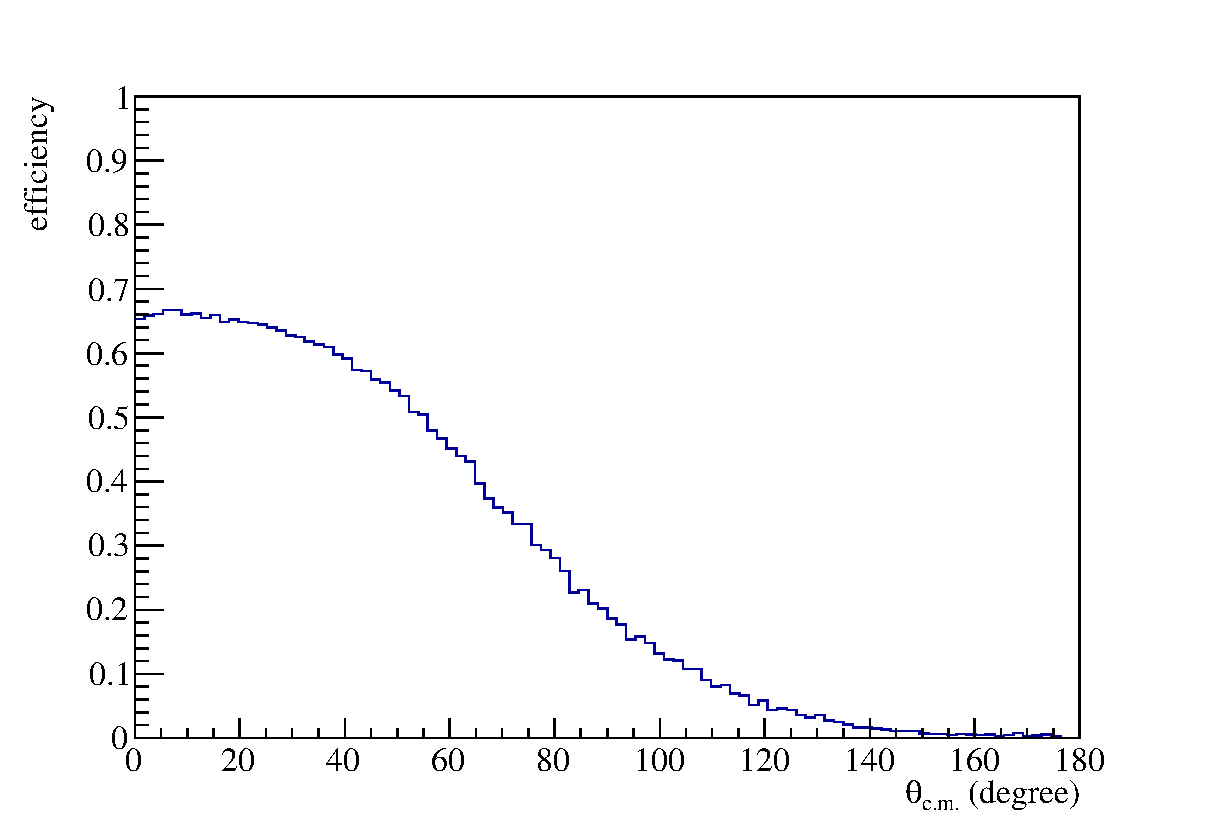
\includegraphics[clip, width=0.8\columnwidth]{detection_efficiency_theta_cm.eps}
  \caption{検出効率の重心系での散乱角依存性.}
  \label{fig::detection_efficiency_theta_cm}
\end{figure}

\section{期待される収量}
Ref.~\cite{takahashietal,kondoetal}によると${}^{12}\mathrm{C}(\mathrm{n},\mathrm{n}'){}^{12}\mathrm{C}(0_{2}^{+})$の
断面積 ($\sigma$) は\SI{8.36}{\milli\barn}である.
OKTAVIAN で現在得られるビーム量 ($N_{\text{b}}$) は最大で$4\pi$に\SI{5e9}{\per\second}である.
この時,半径\SI{10}{\milli\metre}のコリメータからは\SI{1.95e4}{\per\second}の中性子が得られる.
検出効率 ($\varepsilon_{\text{det.}}$) が\SI{48.2}{\percent},
解析効率 ($\varepsilon_{\text{ana.}}$) が\SI{87}{\percent}である.
\isoButaneHydro (\SI{100}{\hecto\pascal}) における${}^{12}\mathrm{C}$の
面密度 ($N_{\text{t}}$) は\SI{1.01e17}{\per\square\milli\metre}である.
%\SI{9.904e-3}{\per\cubic\milli\metre}%\rho = 2.3846e-5\gram\per\cubic\cm
この時,${}^{12}\mathrm{C}(\mathrm{n},\mathrm{n}'){}^{12}\mathrm{C}(0_{2}^{+})$反応の収量は
\begin{align}
  Y &= N_{\text{t}}\times N_{\text{b}}\times \sigma \times\varepsilon_{\text{det.}}\times\varepsilon_{\text{ana.}} \notag\\
  &= \SI{1.01e17}{\per\square\milli\metre}\times\SI{5e9}{\per\second}\times\SI{8.36}{\milli\barn}
  \times\SI{48.2}{\percent}\times\SI{87}{\percent} \notag\\
  &= \SI{6.82e-4}{\per\second}
\end{align}
となる.
12時間の測定で,収量が\num{29.5} events と期待される.

\end{document}
